\chapter{Dynamic multi-objective evolution of classifier ensembles applied to video-based face recognition}

This chapter presents the third and final version of the incremental learning strategy (applied to an AMCS).
While previous work considered only accuracy during the optimization process, this study introduce a multi-objective framework to also consider network structural complexity when evolving a swarm of FAM neural networks and for ensemble selection.
This chapter was submitted for the special edition of the Applied Soft Computing journal on Swarm Intelligence in Image and Video Processing (\cite{connolly12}).

In this chapter, an incremental learning strategy based on particle swarm optimization (PSO) is proposed to efficiently evolve heterogeneous classifier ensembles in response to new reference data.  This strategy is applied to an AMCS where all parameters of a pool of fuzzy ARTMAP (FAM) neural network classifiers  (\emph{i.e.}, a swarm of classifiers), each one corresponding to a particle, are co-optimized such that both error rate and network size are minimized.
To provide a high level of accuracy over time while minimizing the computational complexity, the AMCS integrates information from multiple diverse classifiers, where learning is guided by an aggregated dynamical niching PSO (ADNPSO) algorithm that optimizes networks according both these objectives.
Moreover, pools of FAM networks are evolved to maintain (1) genotype diversity of solutions around local optima in the optimization search space, and (2) phenotype diversity in the objective space.
Accurate and low cost ensembles are thereby designed by selecting classifiers on the basis of accuracy, and both genotype and phenotype diversity. For proof-of-concept validation, the proposed strategy is compared to AMCSs  where incremental learning of FAM networks is guided through mono- and multi-objective optimization.
Performance is assessed in terms of video-based error rate and resource requirements under different incremental learning scenarios, where new data is extracted from real-world video streams (IIT-NRC and MoBo).
Simulation results indicate that the proposed strategy provides a level of accuracy that is comparable to that of using mono-objective optimization (an reference face recognition systems), yet requires a fraction of the computational cost (between 16\% and 20\% of a mono-objective strategy depending on the data base and scenario).

%------------------------------------------------------------------------------%
%------------------------------------------------------------------------------%
\section{Introduction}

%-- Biometric / face recognition -- lack of data
In biometric applications, matching is typically performed by comparing query samples captured with some sensors against biometric models designed with reference samples previously obtained during an enrollment process.
In its most basic form, template matching is performed with biometric models consisting of a set of one or more templates (reference samples) stored in a gallery.
To improve robustness and reduce resources, it may also consists of a statistical representation estimated by training a classifier on reference data.
Neural or statistical classifiers then implicitly define a model of some individual's physiological or behavioral trait by mapping the finite set of reference samples, defined in an input feature space, to an output score or decision space.
Still, the collection and analysis of reference data from individuals is often expensive and time consuming.
Therefore, classifiers are often designed using some prior knowledge of the underlying data distributions, a set of user-defined hyperparameters (\emph{e.g.}, learning rate), and a limited number of reference samples.

%-- Incremental learning
In many biometric applications however, it is possible to acquire new reference samples at some point in time after a classifier has originally been trained and deployed for operations.
Labeled an unlabeled samples can be acquired through re-enrollment sessions, post-analysis of operational data, or enrollment of new individuals in the system, allowing for incremental learning of labeled data and semi-supervised learning of reliable unlabeled data (\cite{jain06, roli08}).
In video-based face recognition, facial images may also be tracked and captured discreetly and without cooperation over a network of IP cameras (\cite{jain06}).
Face acquisition is subject to considerable variations (\emph{e.g.}, illumination, pose, facial expression, orientation and occlusion) due to limited control over unconstrained operational conditions.
In addition, new information, such as input features and new individuals, may suddenly emerge, and underlying data distributions may change dynamically in the classification environment.
The physiology of individuals  (\emph{e.g.}, aging) and operational condition may therefore also change gradually, incrementally, periodically and abruptly over time (\cite{zliobaite10}).
Performance may therefore decline over time as facial models deviate from the actual data distribution (\cite{granger01, poh09, tsymbal08}).

Beyond the need for accurate face recognition techniques in video, efficient classification systems for various real-time applications constitutes a challenging problem.
For instance, video surveillance systems use a growing numbers of IP cameras, and must simultaneously process many video feeds.
The computational burden increases with the number of matching operations, and thus the number of individuals and cameras, frame rate, etc.  

%-- chapter proposal
This chapter seeks to address challenges related to the design of robust adaptive multi-classifier systems (AMCSs) for video face recognition, where facial models may be created and updated over time, as new reference data becomes available.
An incremental learning strategy driven by a dynamic particle swarm optimization (DPSO) and AMCS architecture were previously developed by the authors in (\cite{connolly11}).
In this DPSO-based strategy, each particle corresponds to a fuzzy ARTMAP (FAM) network, and a DPSO algorithm optimizes all classifier parameters (hyperparameters, weights, and architecture) of a swarm of base classifiers such that the error rate.
While adaptation was originally performed only according accuracy with mono-objective optimization, the new strategy and AMCS proposed in this chapter is driven by a new multi-objective aggregated dynamic niching PSO (ADNPSO) algorithm that also considers the structural complexity of FAM networks during adaptation, allowing to design efficient heterogeneous ensembles of classifiers.

This approach also differs with previous work by the authors (\cite{connolly11}) in that a specialized archive is used to capture base classifiers from the swarm and maintain a pool.
To further reduce the computational cost, this archive is constantly modified through time by adding non-dominated classifiers and removing dominated ones with a locally Pareto-optimal criteria.
This locally Pareto-optimal criteria is again used within that pool to select ensembles that are both accurate and with low complexity.

Most techniques in literature are suitable for designing classification systems with an adequate number of samples acquired from ideal environments, where class distributions remain unchanged over time. However, classifier ensembles are well suited for adaptation in changing environments. Adaptive ensemble-based techniques like Learn++ (\cite{polikar01}) and other Boosting variants, where a new classifier is trained independently for new samples, and classifiers are weighted such that one criteria is maximized (classification accuracy on recent data), may provide a robust approach (\cite{minku10}). Other approaches discard classifiers when they become inaccurate or concept change is detected (\cite{nishida08}), although maintaining a pool with these classifiers allows to handle recurrent change. Moreover, methods that rely exclusively on adding new ensemble members become problematic if all classes are not represented within the new data. With the current face recognition application, for instance, when new data becomes available after a classifier is designed and deployed in the field, it will most likely belong to one or few individuals at a time. Previously-trained classifiers will not recognize new classes, classifiers trained with the new data will not recognize older classes.

%-- Context
The proposed ADNPSO strategy evolves a pool of incremental learning FAM classifiers, and may refine and add classes on the fly.
To increase the performance of an heterogeneous ensembles, this strategy seeks to maintain diversify among the base classifiers during generation and evolution of pools, and during ensemble selection, according to several criteria.
This chapter focuses on video-based face recognition applications in which two incremental learning scenarios may occur -- enrollment (initial design) and update of facial models.
Performance of AMCSs is assessed in terms of classification rate and resource requirements for incremental learning of new data blocks from two real-world video data sets -- Institute of Information Technology of the Canadian National Research Council (IIT-NRC) (\cite{gorodnichy05}) and Motion of Body (MoBo) (\cite{gross02}).
In experiments, the AMCS performs biometric identification of facial regions against the model of individuals in closed-set (1-against-$K$) identification, as found in access control applications.

%-- Structure
The next section provides an overview of the state-of-the-art in adaptive biometrics and a general biometric system for video-based face recognition system.
In Section \ref{sec:c3_adaptation}, the AMCS framework considered in this chapter is described, focusing on the relationship between the classification environment (where the FAM networks learn reference data), and the optimization environment (where particles evolve).
The new incremental learning strategy used (including ADNPSO algorithm and specialized archive) to evolve the AMCS are presented in Section \ref{sec:c3_algo}.
The data bases, incremental learning scenarios, protocol, and performance measures used for proof-of-concept simulations are described in Section \ref{sec:c3_methodology}.
Finally, experimental results are presented and discussed in Section \ref{sec:c3_res_dis}.

%------------------------------------------------------------------------------%
%------------------------------------------------------------------------------%
%------------------------------------------------------------------------------%
\section{Adaptive biometrics and video face recognition}
\label{sec:c3_app}

%-- Statement
The main problem addressed in this chapter is the design of accurate and efficient adaptive systems to perform video-to-video face recognition, where video sequences are used for building the facial model of each individual during the learning phase.
Adaptive systems have been proposed in the literature to refine biometric models for different traits (\emph{e.g.}, face, fingerprints, etc.) according to the intra-class variations in input samples (\cite{roli08}).
With self-adaptive or semi-supervised learning strategies, biometric models are initially designed during enrollment using labeled training data, and then updated with highly confident unlabeled data obtained during operations (\cite{poh09, rattani10}).
These strategies are however vulnerable to outliers, dispersion and overlap in class distributions.
Stringent criteria are required for selection of highly confident data, to minimize the probability of introducing impostor data into updated biometric models.

On the other hand, systems have used newly-acquired labeled reference samples to update the selection of user template from a gallery via clustering and editing techniques (\cite{uludag04}), and have performed on-line learning of genuine samples over time to update each user's single super template (\cite{jiang02}).
It is however difficult to represent intra-class variations with a single template (\cite{roli08}).
In either case, the biometric model of an individual tends to diverge from its underlying class distribution due to the limited reference data, complexity, and changes in the classification environment.
In their efforts to avoid model corruption and to maintain a high level of accuracy, classifiers adapted incrementally over time tend to become complex (\cite{connolly11}).

Biometric systems specifically designed for the recognition of faces in video streams are relevant in different scenarios and applications.
Applications of video-based face recognition range from open-set video surveillance, where individuals enrolled to a watch list are recognized among other unknown people in dense and moving crowds (\cite{ekenel09}), to closed-set identification or verification for access control applications, where individuals enrolled to a system are authenticated prior to accessing secured resources, possibly in conjunction with a password, access card, etc. (\cite{stallkamp07}).
In this chapter, video-based face recognition is considered for closed-set identification applications.

In addition to difficulties mentioned earlier, video-based face recognition remains a very challenging problem since faces captured in video frames are typically low quality and generally small.
The design of efficient systems for facial matching involves a trade-off between classification speed, accuracy and resources for storage of facial models.
In video-based face recognition, fast classification is often required to process facial regions at near real-time processing (captured at 30 frames/second in each video feed).
It is well-known that state-of-the-art systems are confronted with complex environments that change during operations, and their facial models are designed during a preliminary enrollment process, using limited data and knowledge of individuals.
The need to design and store representative facial models for recognition -- be it with more user templates or a statistical representation -- increases the resource requirements of the system.

A typical approach used to recognize faces in video streams consists in exploiting only spatial appearance information, and applying extensions of still image techniques on high quality facial regions captured through segmentation (\cite{matta09}).
Several powerful techniques proposed to recognize faces in static 2D images are described in \cite{zhang09,zhao03}.
The predominant techniques are the same used to represent faces in static 2D images: appearance-based methods like Eigenfaces, and feature-based methods like Elastic Bunch Graph Matching (\cite{zhang09,zhao03}).
However, the performance of these techniques may degrade considerably when applied for video-based face recognition in unconstrained scenes.
To reduce matching ambiguity and provide a higher level of accuracy, face recognition applications specifically designed toward video sequences combine spatial and temporal information contained in video streams (\cite{edwards99}).

In this chapter, it is assumed that a track-and-classify system is used to accumulate the responses of a classifier using kinematic information of faces in a scene (\cite{matta09}).
Figure \ref{fig:c3_faceRec} depicts a general track-and-classify for spatio-temporal recognition of faces in video.
It is assumed that 2D images in the video streams of an external 3D scene are captured using one or more IP or network cameras.

%--------------------------- Face recognition system --------------------------%
\begin{figure*}[t] \centering
  \fbox{
  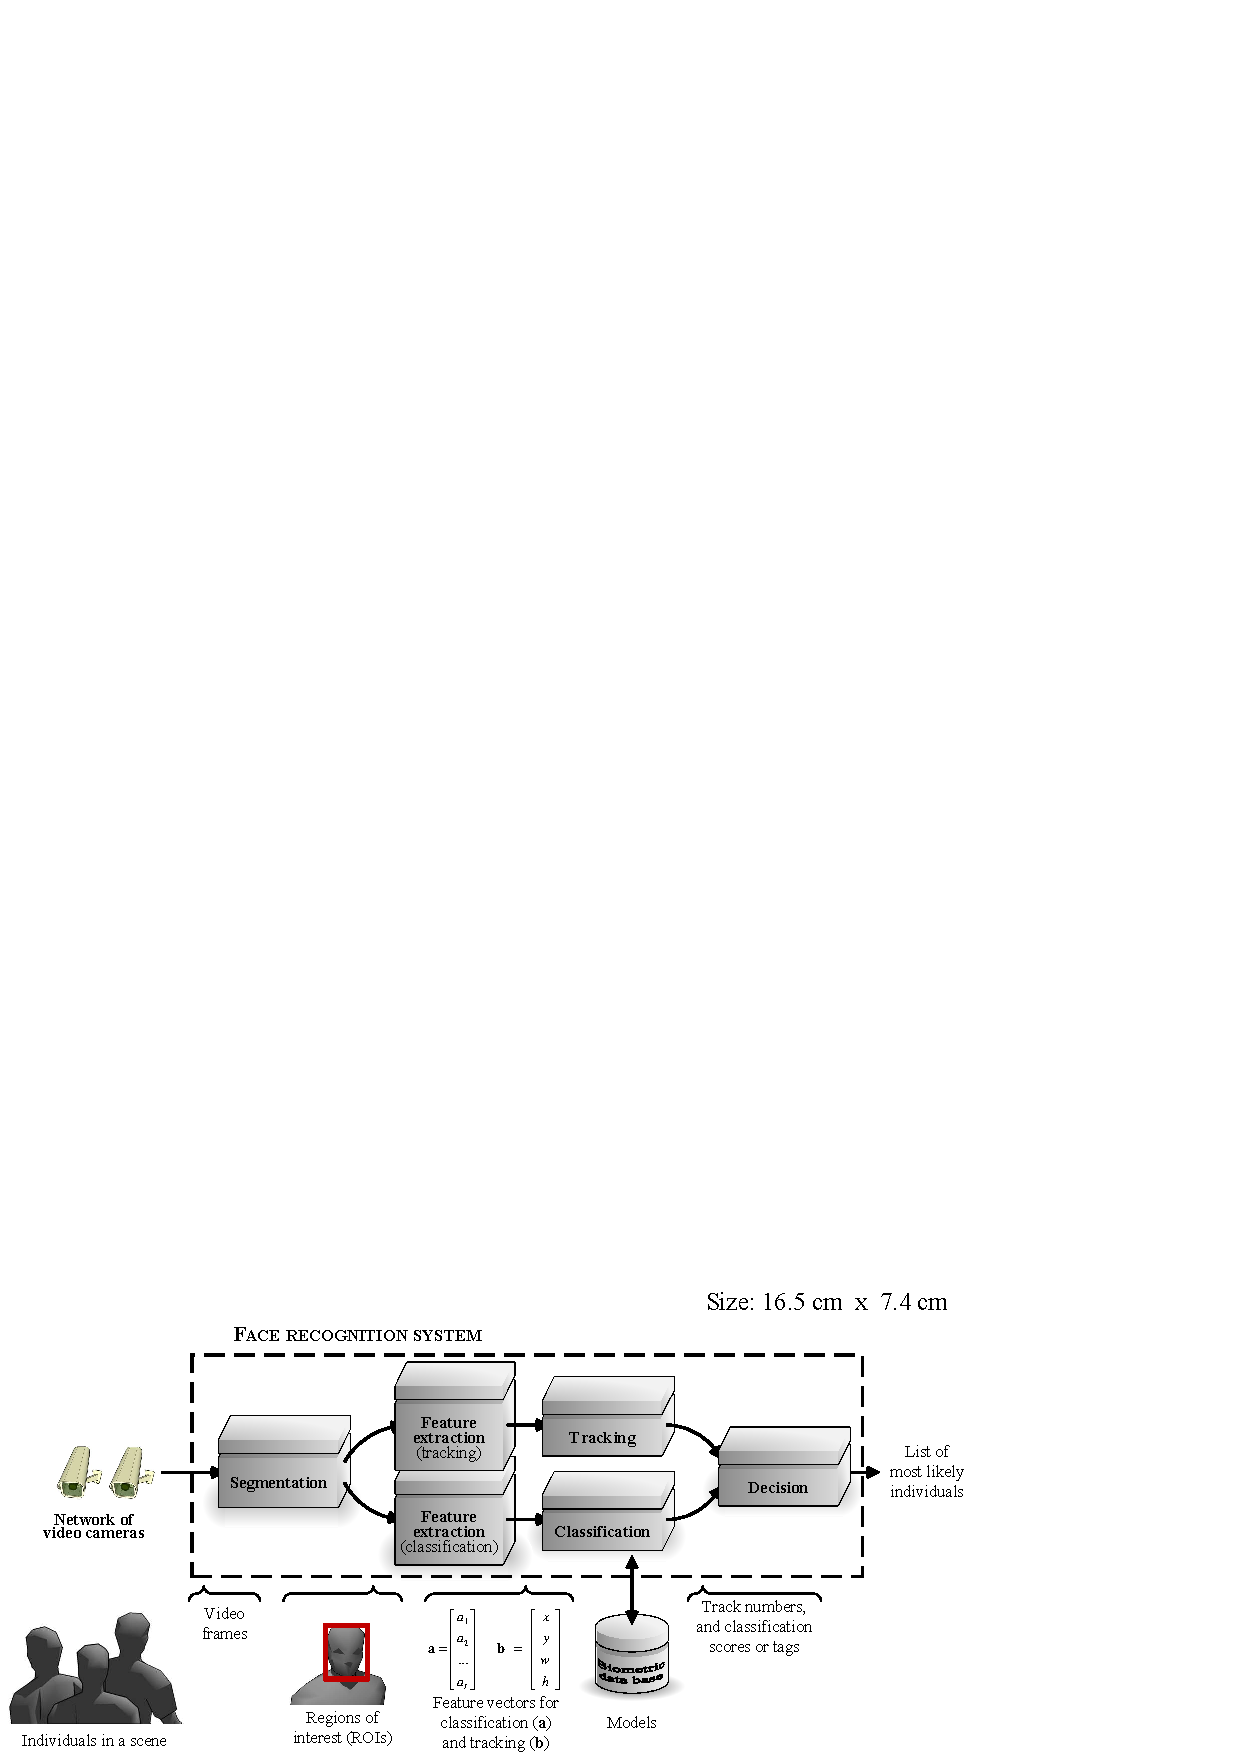
\includegraphics[width =0.97\linewidth, viewport= 0cm 0cm 16.5cm 7.4cm, clip]
 		              {c3_fig2} }
  \caption{A generic track-and-classify biometric system for video-based face recognition}
	\label{fig:c3_faceRec}
\end{figure*}
%-------------------------- /Face recognition system --------------------------%

First, the system performs segmentation to locate and isolate regions of interest (ROIs) corresponding to the faces in a frame.
From the ROIs, features are extracted for tracking and classification.
The tracking features can be the position, speed, acceleration, and track number assigned to each ROI on the scene so that the tracker may follow the movement or expression of faces across video frames (\cite{granger01}).
On the other hand, classifiers will require invariant and discriminant classification features extracted from the ROIs so that the classification module may match input feature patterns, mapped in an $\mathbb{R}^I$ input feature space, to the face models of individuals enrolled to the system.
Facial matching may be implemented with templates, statistical, or neural pattern classifiers.
With neural network classifiers, for instance, the facial model of individuals by the hyperparameters, synaptic weights, and architecture estimated during training.

Finally, the decision module may integrate the responses from the tracking and classification modules over several video frames.
If the decision module employs a track-and-classify approach, the facial regions are presented to the face recognition system and predictions for each ROI are accumulated over time according to the facial trajectories defined by the tracker.
With identification and surveillance applications for instance, ambiguity is reduced by accumulating responses (classification scores) over several frames over the trajectory of each individual in the scene, thus improving accuracy and robustness of face recognition in video (\cite{barry07}).

Although the current chapter uses a track-and-classify architecture other methods exist for spatio-temporal recognition in video sequences.
Head and facial motion during the sequence can be exploited by either estimating the optical flow or tracking a few facial landmarks over time with a template matching strategy.
Temporal dynamics and statistics of training video sequences can also be modeled using Hidden Markov Models, particle filters, or time series state space models.
A probabilistic appearance manifold approach can also be used to exploit temporal information of each successive frame in a video sequence.
Bayesian inference then allows to include temporal coherence in distance calculation during recognition.
A review of recent techniques for spatio-temporal face recognition for video sequences can be found in \cite{matta09}.

With most systems for video face recognition, conditions for data acquisition are typically considered to be constrained, and the physiology of individuals and operational condition do not change over time. Systems are designed a priori, during a preliminary enrollment phase, but the number of reference samples and knowledge of class distributions are limited. 
Adapting the system in response to new reference data may allow to maintain a high level of performance by reducing the divergence over time between facial models and underlying data distributions in the real-world environments. However, most classification techniques used for face matching would require training from the start using all previously acquired data through supervised batch learning. 

In the next section an ADNPSO strategy is proposed  for supervised incremental learning allows to enroll and update the facial model of individuals from video streams after the face recognition system has been deployed for operations. Efficient incremental learning is an undisputed asset as the memory and time complexity associated with storing and training is greatly reduced. 
The objective of this new ADNPSO strategy is to evolve classifiers according to both accuracy and network size, leading to more accurate and reliable systems that perform efficient matching of captured facial regions.

%------------------------------------------------------------------------------%
%------------------------------------------------------------------------------%
%------------------------------------------------------------------------------%
\section{Adaptive classifier ensembles}
\label{sec:c3_adaptation}

Adapting facial models in changing classification environments, such as required for enrollment or update in video face recognition, raises the so-called stability-plasticity dilemma, where stability refers to retaining existing and relevant knowledge while plasticity enables learning new knowledge (\cite{grossberg88}).
Since ensemble based methods allow to exploit multiple and diverse views of a problem, they have been shown to be efficient in such cases, where concepts (\emph{i.e.}, underlying data distributions) change in time (\cite{minku10}).

For a wide range of applications, where adaptation is not necessarily required, classifier ensembles allow to exploit several views of a same problem to improve the overall accuracy and reliability.
Recently, various methods employing adaptive ensembles of classifiers have been proposed to perform incremental learning (\cite{kapp10, polikar01}).
With the use of a combination function, they also offer a flexibility over single classifiers in how class models can be managed and adapted.

These methods can be divided in three general categories (\cite{kuncheva04}).
Dynamic combination, or ``horse racing'', methods where individual base classifiers are trained in advance to form a fixed ensemble where only the combination rules is changed dynamically (\cite{blum97, widmer96, xingquan04}).
Second, methods that rely on new data to update the parameters of ensemble base classifiers an online learner (\cite{gama04}).
If blocks of data are available, training can also be performed in batch mode while changing or not the the combination rule at the same time (\cite{breiman99, ganti02, oza01, wang03}).
The last main category consists of methods that grow ensembles by adding new base classifiers and replacing old or underperforming ones when new data is available (\cite{chen01, kolter07, street01, tsymbal08}).
Finally there are adaptive ensembles that use hybrid approaches that combine adding new base classifiers and adjusting the combination rule to update class models.
The most notable are streaming random forests with entropy (\cite{abdulsalam11}), Hoeffding tree with Kalman filter-based active change detection using adaptive sliding window (\cite{bifet10}), maintaining and choosing the better of two ensembles trained with current and old data (\cite{scholz06}), and the AdaBoost-like Learn++ (\cite{polikar01}).

Among these methods, horse racing approaches cannot accommodate new knowledge since base classifiers in the ensemble are never updated with new data.
On the other hand, while online learners and growing ensembles can be used to explore unknown regions of the feature space, and focus on the issue of concept drift, where underlying class distributions changes in time.
They often train and combine new classifiers to a pool without updating pre-existing classifiers at the risk of corrupting older knowledge.
While these classifiers are trained with new data, their plasticity (or learning dynamics) tends to remain fixed throughout the learning process, without being adjusted to accommodate new knowledge.
Video face recognition systems in unconstrained scenes are often faced with recurring changes regarding the environment (\emph{e.g.}, light effect over the course of a day) and the individuals to recognize (\emph{e.g.}, glasses).
Since few reference samples are available, hidden concepts are often revealed  (different known view points from a sensor or of a trait).

In practice, when new reference data becomes available during operations, it will most likely incorporate sampled captured from one or few individuals at a time.
With growing ensembles, previously-trained classifiers will not be able to integrate new classes, and the new ones (trained with the new reference data) will represent only facial models of the latest individuals registered to the system.

%-------------------------------- Environments --------------------------------%
\begin{figure*}[tb]
  \centering
  \fbox{
  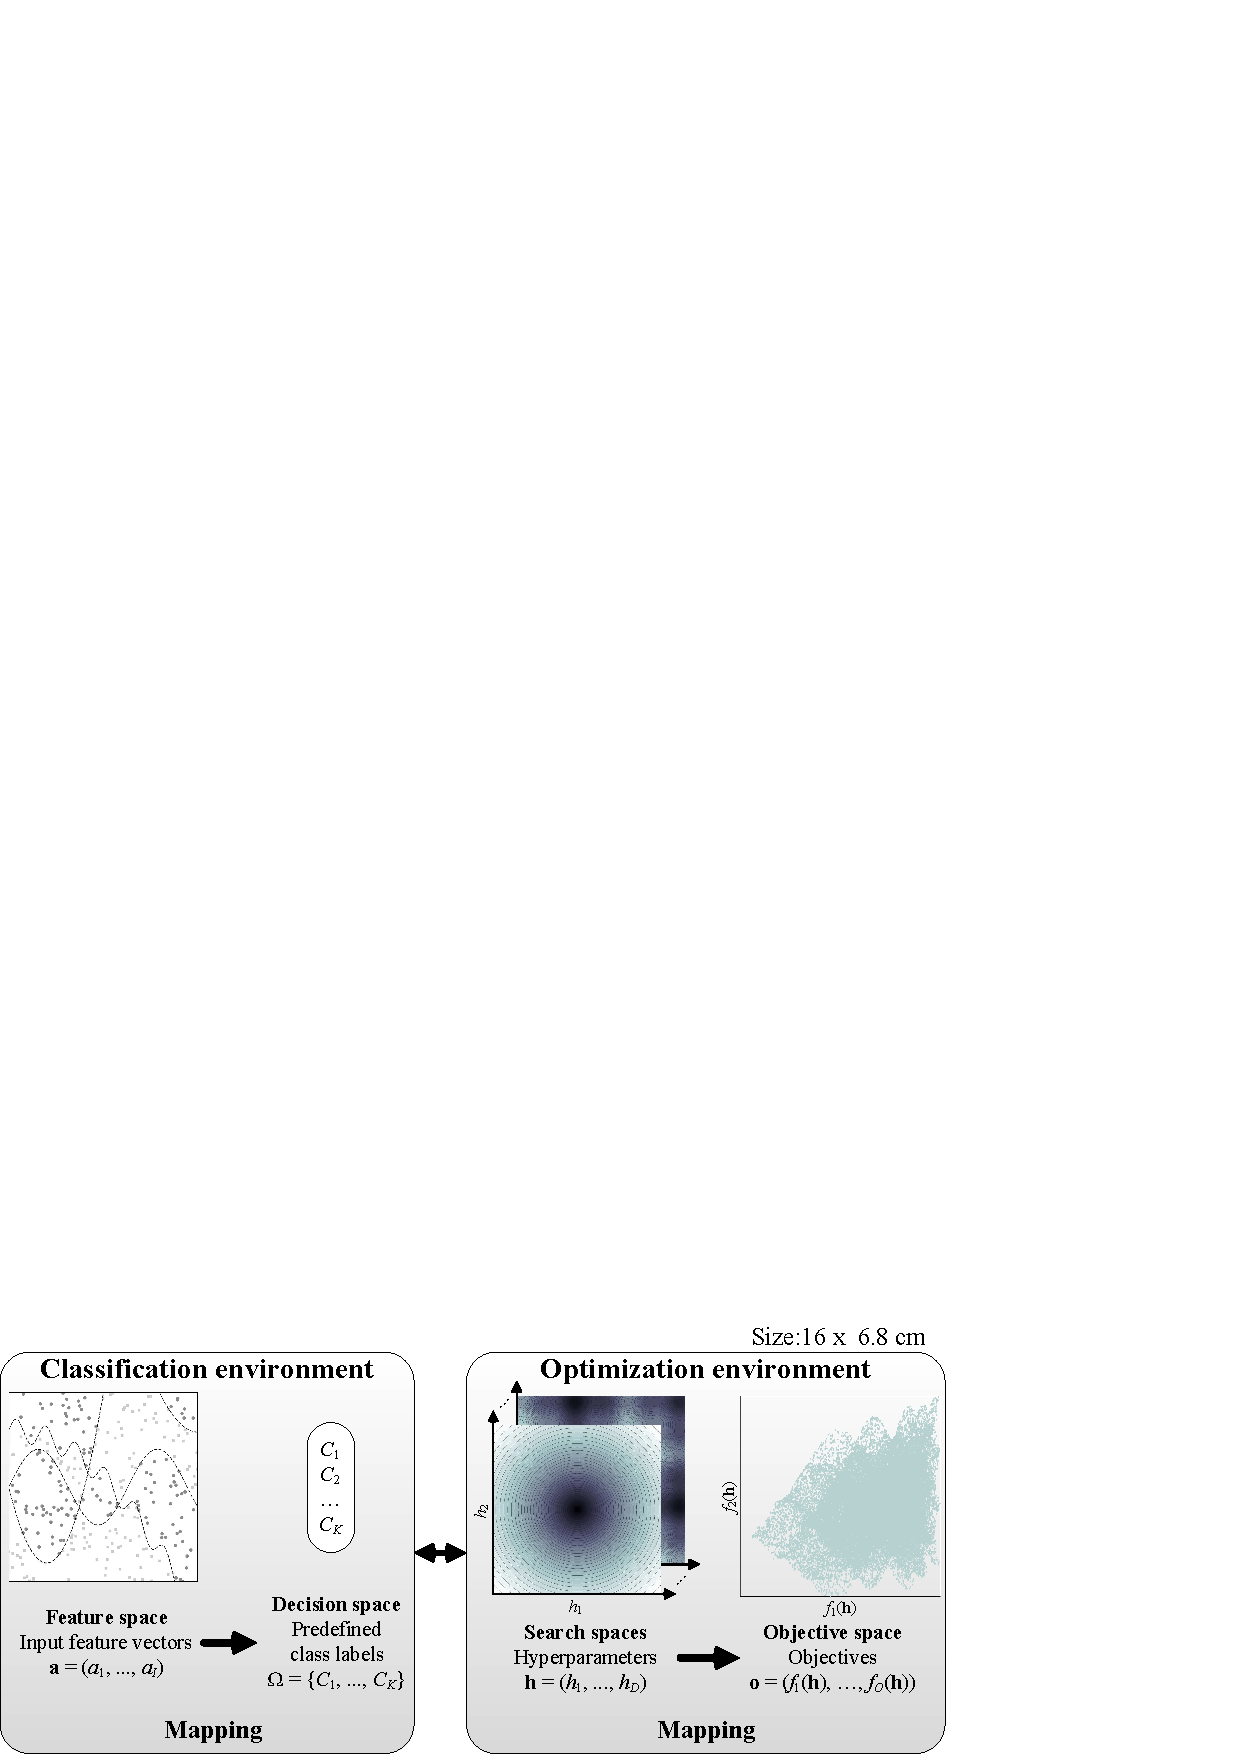
\includegraphics[width=0.9\linewidth, viewport=0cm 0cm 16.cm 6.81cm, clip]
                  {c3_fig1} }
  \caption{Pattern classification systems may be defined according to two environments.
A \emph{classification environment} that maps a $\mathbb{R}^I$ input feature space to a decision space, respectively defined by feature vectors \textbf{a}, and a set of class labels $C_k$.
As classifier learning dynamics is governed by a vector \textbf{h} of hyperparameters, the latter interacts with an \emph{optimization environment}, where each value of \textbf{h} indicates a position in several search spaces, each one defined by an objective considered during the learning process.
For several objective functions (each corresponding to a search space), solutions (trained FAM networks) can be projected in an objective space}
	\label{fig:c3_environments}
\end{figure*}
%------------------------------- \Environments --------------------------------%

%-- Previous work
In previous work, the authors have proposed an adaptive multiclassifier system (AMCS) that is driven by a strategy based on dynamic particle swarm optimization (DPSO) for supervised incremental learning for the design and update of facial biometric models (\cite{connolly11}).
Given its capabilities to perform supervised incremental learning of limited data, and to efficiently match of query samples to facial models in the system, the Fuzzy ARTMAP (FAM) neural networks is used as the ensemble's base classifier.
Using DPSO and a cooperative neural network co-evolution paradigm (\cite{potter00}), the incremental learning strategy is applied to the optimization of a swarm of FAM networks in the hyperparameter search space.
As illustrated in Figure \ref{fig:c3_environments}, DPSO explores the hyperparameter search spaces and guides a swarm of different FAM classifiers.
They are trained on the same data, but using different learning dynamics, \emph{i.e.}, different hyperparameter settings.
This process yields an \emph{heterogeneous}\footnote{This definition of heterogeneous ensembles differs with respect to certain others found in literature.
In this chapter, they are defined as similar classifiers that learn different data sets, or classifiers of different types train on the same data (\cite{oliveira09, rashid09}).}
 pool of classifiers that is diversified in both feature and decision spaces (\cite{valentini03}).
When new labeled reference data becomes available from the operational environment, classifier ensembles evolve to design new facial models or update existing ones.
Since this approach does not directly optimize FAM parameters (\emph{i.e.}, synaptic weights for neural networks), and can be applied other classifiers.
Other examples showing how particle swarm optimization algorithms are applied in this manner are summarizes in \cite{granger10, kapp10}.

By applying the DPSO strategy within an adaptive classification system (ACS), the authors have previously shown that to perform incremental learning with constructive classifiers such as FAM networks, some of the older data must be stored in memory so that old and still valid knowledge is not overshadowed by newer concepts corresponding to incoming reference data (\cite{connolly10}).
They have also shown that optimizing FAM learning dynamics according to accuracy during supervised incremental learning corresponds to a dynamic mono-objective optimization problem (\cite{connolly10}).
Within the AMCS, the authors have then verified that with FAM networks, \emph{genotype} (\emph{i.e.}, hyperparameter) diversity among solutions in the search space leads to ensemble diversity in the feature and decision spaces (\cite{connolly11}).
Although these AMCSs provide a high level of accuracy and robustness when only limited data is available, FAM networks are generated through mono-objective optimization of accuracy, and become structurally complex over time, as new data is learned.

%%------------------------------------------------------------------------------%
%------------------------------------------------------------------------------%
\subsection{An adaptive multiclassifier system}
\label{sec:c3_AMCS}

Figure \ref{fig:c3_amcs} depicts the evolution of an AMCS performing incremental learning of new data.
It is composed of (1) a long term memory (LTM) that stores and manages incoming data for validation, (2) a population of base classifiers, each one suitable for supervised incremental learning, (3) a dynamic population-based optimization module that tunes the user-defined hyperparameters of each classifier, (4) a specialized archive to keep a pool of classifiers for ensemble selection, and (5) an ensemble selection and fusion module.
This system differs from the AMCS presented in \cite{connolly11} in that the optimization module now performs multi-objective (rather than mono-objective) optimization, and the pool of classifiers, from which ensembles selection is performed, is now an archive that is filled during the multi-objective optimization (MOO) process.

%------------------------- Framework - for section 2 --------------------------%
\begin{figure*}[t]
  \centering
  \fbox{
  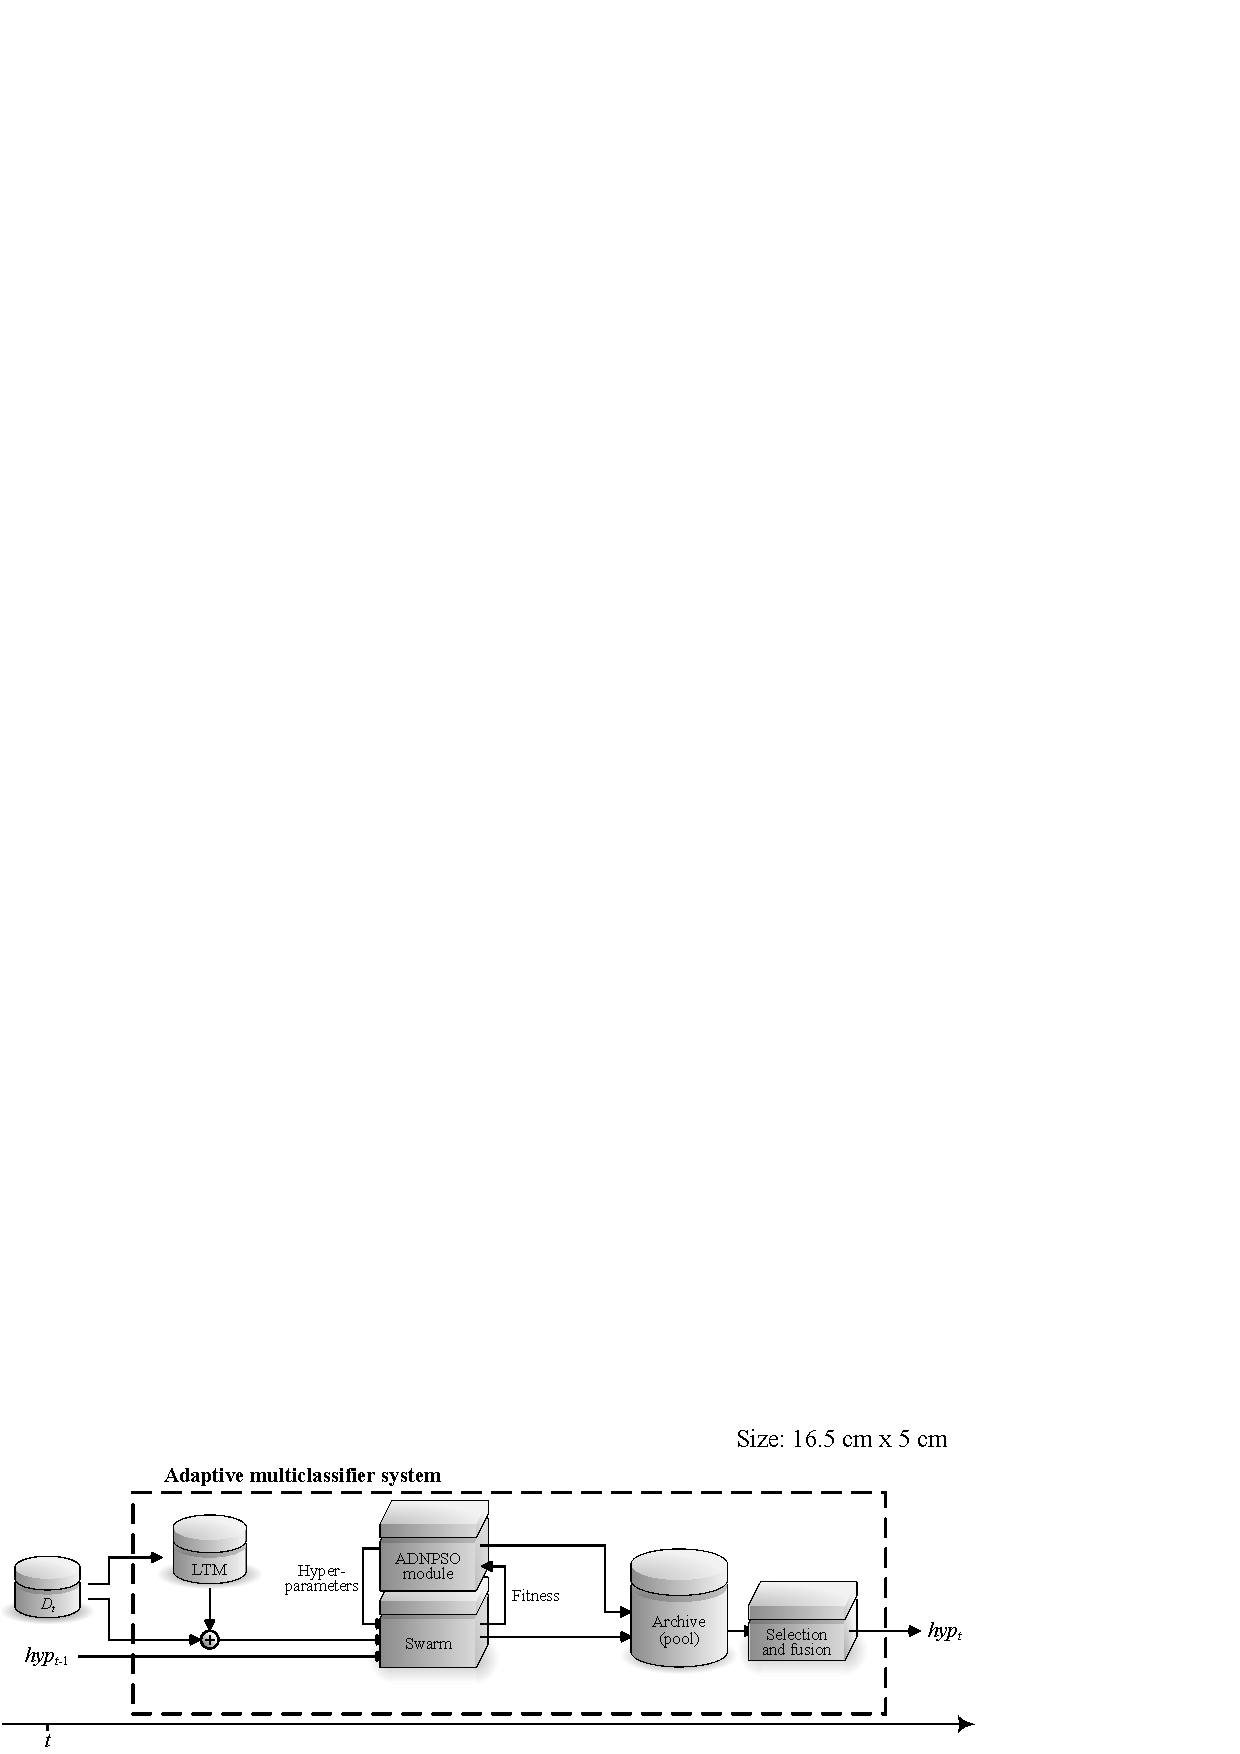
\includegraphics[width =0.97\linewidth, viewport =0cm 0cm 16.5cm 5cm, clip]
  								{c3_fig3} }
  \caption{Evolution over time of the adaptive multiclassifier system (AMCS) in a generic incremental learning scenario, where new blocks of data are used to update a swarm of classifiers.
Let $D_1$, $D_2$, ... be blocks of training data that become available at different instants in time $t=1,2,...$.
The AMCS starts with an initial hypothesis $hyp_0$ according to the prior knowledge of the classification environment.
On the basis of new data blocks $D_t$, each hypothesis $hyp_{t-1}$ are updated to $hyp_t$ by the AMCS}
	\label{fig:c3_amcs}
\end{figure*}
%------------------------- \Framework - for section 2 -------------------------%

When a new block of learning data $D_t$ becomes available to the system at a discrete time $t$, it is employed to update the LTM, and evolve the swarm of incremental classifiers (see Figure \ref{fig:c3_amcs}).
Each FAM network is associated to a particle in an hyperparameter search space, and a DPSO module, through a DPSO-based learning strategy, conjointly determines the classifiers hyperparameters, architecture, and parameters such that FAM networks error rate \emph{and} size are minimized.
A specialized archive stores a pool of classifiers, corresponding to locally non-dominated solutions (of different structural complexity) found during the optimization process.
Once the optimization process is complete, the selection and fusion module produces a heterogeneous ensemble by selecting classifiers from the archive (or pool), based on their accuracy, genotype, and phenotype diversity.
It then combines them with a simple majority vote.
The LTM stores reference samples from each individual for cross-validation during incremental learning and fitness estimation of particles on the objective function (\cite{connolly10}).
Data from $D_t$ is partitioned and combined with that of the LTM to create three subsets: a training data set $D_t^\text{t}$, a validation data set $D_t^\text{v}$, and a fitness estimation data set $D_t^\text{f}$. 

In this chapter, a particular realization of this AMCS is considered.
FAM neural networks (\cite{carpenter92}) are employed to implement the swarm of incremental learning classifiers and a new ADNPSO algorithm is used for optimization according to multiple objectives.
The rest of this section provides additional details on the FAM and on the optimization module.
The ADNPSO algorithm, specialized archive, and selection and fusion modules are discussed in Section \ref{sec:c3_algo} along with the ADNPSO incremental learning strategy.

%------------------------------------------------------------------------------%
%------------------------------------------------------------------------------%
\subsection{Fuzzy ARTMAP neural network classifiers}
\label{sec:c3_fam}

ARTMAP refers to a family of self-organizing neural network architectures that is capable of fast, stable, on-line, unsupervised or supervised, incremental learning, classification, and prediction.
A key feature of these networks is their unique solution to the stability-plasticity dilemma.
The fuzzy ARTMAP (FAM) integrates the unsupervised fuzzy ART neural network to process both analog and binary-valued input patterns into the original ARTMAP architecture (\cite{carpenter92}).
Matching ROIs (represented with appearance pattern \textbf{a}) against the facial model of individuals enrolled to a face recognition system is typically the bottleneck, especially as the number of individuals grows, and the FAM classifier is used because it can perform supervised incremental learning of limited data for fast and efficient matching.
The facial models are learned a priori (during training) by estimating the FAM weights, architecture and hyperparameters of each individual (\emph{i.e.}, output class) enrolled to the system. 

The fuzzy ART neural network consists of two fully connected layers of nodes: a $2I$ node input layer $F_1$ to accommodate complement-coded input patterns, and a $J$ node competitive layer, $F_2$.
A set of real-valued weights ${\bf W} = \{w_{ij} \in [0,1] : i = 1, 2, ..., 2I;\, j = 1, 2, ..., J\}$ is associated with the $F_1$-to-$F_2$ layer connections.
The $F_2$ layer is connected, through learned associative links, to an output $K$ node map field $F_{ab}$, where $K$ is the number of classes in the decision space.
With FAM, a set of binary weights ${\bf W}^{ab} = \{w^{ab}_{jk} \in \{0,1\} : j = 1, 2, ..., J;\, k = 1, 2, ..., K\}$ is associated with the $F_2$-to-$F_{ab}$ connections.
Each $F_2$ node $j = 1, ... , J$ corresponds to a category that learns a prototype vector ${\bf w}_j = (w_{1j}, w_{2j},..., w_{2Ij})$, and is associate with one of the output classes $k=1,...,K$.
During the training phase, FAM dynamics is governed by four hyper-parameters: the choice parameter $\alpha>0$, the learning parameter $\beta \in \left[ 0,1 \right]$, the baseline vigilance parameter $\bar{\rho} \in \left[ 0,1 \right]$, and the match-tracking parameter $\epsilon  \in [-1,1]$.
For incremental learning, FAM is able to adjust previously-learned categories, in response to familiar inputs, and to create new categories dynamically in response to inputs different enough from those already seen.

The following describes fuzzy ARTMAP during supervised learning of a finite data set.
When an input pattern ${\bf a} = (a_1,...,a_I)$ is presented to the network and the vigilance parameter $\rho \in \left[ 0,1 \right]$ is set to its baseline value $\bar{\rho}$. The input pattern ${\bf a}$ is complement-coded to make a $2I$ dimensions network's input pattern: ${\bf A} = ({\bf a},{\bf a}^{c}) = (a_1, a_2, ..., a_I; a^c_1, a^c_2, ..., a^c_I)$, where $a^c_i = (1-a_i)$, and $a_i \in [0,1]$. Each $F_2$ node is activated according to the \emph{Weber law choice function}:
\begin{equation}\label{eq:c3_choice}
	T_j({\bf A}) = |{\bf A} \wedge {\bf w}_j| / (\alpha + |{\bf w}_j|),
\end{equation}  and the node with the strongest activation $j^* = \text{argmax}\left\{T_j:j=1,...,J\right\}$ is chosen.
The algorithm then verifies if ${\bf w}_{j^*}$ is similar enough to ${\bf A}$ using the vigilance test:
\begin{equation}
	|{\bf A} \wedge {\bf w}_{j^*}| / 2I \geq \rho.
\end{equation}
If node $j^*$ fails the vigilance test, it is deactivated and the network searches for the next best node on the $F_2$ layer.
If the vigilance test is passed, then the map field $F^{ab}$ is activated through the category $j^*$ and FAM makes a class prediction $k^* = k(j^*)$.
In the case of an incorrect class prediction $k^*=k(j^*)$, a match tracking signal adjusts $\rho = \left(|{\bf A} \wedge {\bf w}_{j^*}| / 2I\right)+ \epsilon$. Node $j^*$ is deactivated, and the search among $F_2$ nodes begins anew. If node $j^*$ passes the vigilance test, and makes the correct prediction, its category is updated by adjusting its prototype vector ${\bf w}_{j^*}$ to:
\begin{equation}
{\bf w}_{j^*}' = \beta({\bf A} \wedge {\bf w}_{j^*}) + (1 - \beta){\bf w}_{j^*}.
\end{equation}
On the other hand, if none of the nodes can satisfy both conditions (vigilance test and correct prediction), then a new $F_2$ node is initialed. This new node is assigned to class $K$ by setting $w^{ab}_{j^*k}$ to 1 if $k=k^*$ and 0 otherwise, and ${\bf w}_{j^*}'=\textbf{A}$.

Once the weights ${\bf W}$ and ${\bf W}^{ab}$ have been found through this process, the fuzzy ARTMAP can predict a class label from an input pattern by activating the best $F_2$ node $j^*$, which activates a class $k^*=k(j^*)$ on the $F_{ab}$ layer.
Predictions are obtained without vigilance and match tests. 
During operation, time and memory complexity of FAM are proportional its structural complexity and depends heavily on the number of $F_1$ and $F_2$ layer nodes.
To perform predictions given an input pattern of $I$ features $F_1$ layer and an $F_2$ layer of $J$ nodes, FAM networks complement code the $I$ features, compute the choice function for the $J$ category prototypes, leading to a worst-case time and memory complexity per input sample of $O(IJ)$.
During incremental learning, the $F_2$ layer tends to grow depending on the hyperparameter values, the number of reference samples, and the geometry of the underlying data distributions.
In the worst case, FAM will memorize the training data set, and create one $F_2$ category node per reference sample.
In this chapter, it is assumed that incremental learning of new data is not performed on-line, but in a relatively short time frame.

A standard vector of hyperparameters $\textbf{h}_\text{std} = (\alpha = 0.001, \beta=1, \epsilon=0.001, \bar{\rho}=0)$ is commonly fixed to minimize network structural complexity (\cite{carpenter92}).
The authors have shown that by adjusting these hyperparameters, it is possible to adapt FAM learning dynamics with regards to currently available training data (\cite{connolly10, connolly11, granger07}).
It is possible to generate heterogeneous pools of classifiers (\cite{connolly10_2}).
Moreover, they have also verified the amount of diversity among hyperparameter vectors $\textbf{h}$ of each classifier is correlated with the amount of diversity within a pool of classifier (\cite{connolly11}).
Using these results, the authors generate a pool of diversified FAM networks, and select ensembles among that pool for improved generalization capabilities.
However, since these ensembles where created through a mono-objective optimization process focused only on accuracy, each network of the pool tends to create several prototype categories when learning new data, leading to a considerable computational cost.

%------------------------------------------------------------------------------%
%------------------------------------------------------------------------------%
\subsection{Adaptation as a dynamic MOO problem}

In this chapter, the AMCS optimization module will seek to find the hyperparameters vector $\textbf{h}=\left(\alpha, \beta, \epsilon, \bar{\rho}\right)$ that seeks to maximize FAM accuracy while minimizing network structural complexity, that is: 
\begin{equation}  \label{eq:c3_dmoop}
	\begin{split}
		 \textnormal{minimize} &  \left\{ \textbf{f}(\textbf{h},t):= [f_e(\textbf{h},t), f_s(\textbf{h},t)]\ |\ 		
												\textbf{h}\in\mathbb{R}^4, t\in\mathbb{N}_1 \right\},
%		 \textnormal{minimize} &  \left\{ f_s(\textbf{h},t)\ |\ 		
%												\textbf{h}\in\mathbb{R}^4, t\in\mathbb{N}_1 \right\},
	\end{split}
\end{equation}
where $f_e(\mathbf{h},t)$ is the generalization error rate and $f_s(\mathbf{h},t)$ is the size of the $F_2$ layer (\emph{i.e.}, number of $F_2$ nodes) of the FAM network for a given hyperparameter vector $\textbf{h}$, and after learning data set $D_t$ incrementally at a discreet time $t$ (\cite{connolly10}).
In this context, it has been shown that adapting the FAM classifier's hyperparameters vector $\textbf{h}=\left(\alpha, \beta, \epsilon, \bar{\rho}\right)$ according to $f_e(\mathbf{h},t)$ corresponds to a dynamic mono-objective optimization problem (\cite{connolly10}).
More precisely, it constitutes a type III optimization environment, where both the location and value of optima positions change in time (\cite{engelbrecht05}).
Although it was not explicitly verified, it is assumed that training FAM with different values of \textbf{h} leads to different number of FAM $F_2$ nodes and that the objective function $f_s(\textbf{h},t)$ also correspond to a type III optimization environment.
Still it is sufficient that only one of the objectives does so for the entire optimization problem to be considered dynamic.

As a MOO problem, the first goal of the optimization module is to find the Pareto front of non-dominated solutions according to several objectives (see Figure \ref{fig:c3_pareto}).
Given the set of objectives $\mathbf{o}$ to minimize, a vector $\textbf{h}^d$ in the hyperparameter space is said to \emph{dominate} another vector $\textbf{h}$ if (see Figure \ref{fig:c3_dominance}):
\begin{equation}  \label{eq:c3_dom}
	\begin{split}
		&\forall o \in \mathbf{o}: f_o(\textbf{h}^d) \leq f_o(\textbf{h})
			\text{, and}\\
		&\exists o \in \mathbf{o}: f_o(\textbf{h}^d) < f_o(\textbf{h}).
	\end{split}
\end{equation}
The Pareto optimal set, defining a Pareto front, is the set of non-dominated solutions (Figure \ref{fig:c3_parFront}).

%---------------------------------- Dominance ---------------------------------%
\begin{figure*}[t]
  \centering
  \fbox{
  \subfloat[Dominance]{ 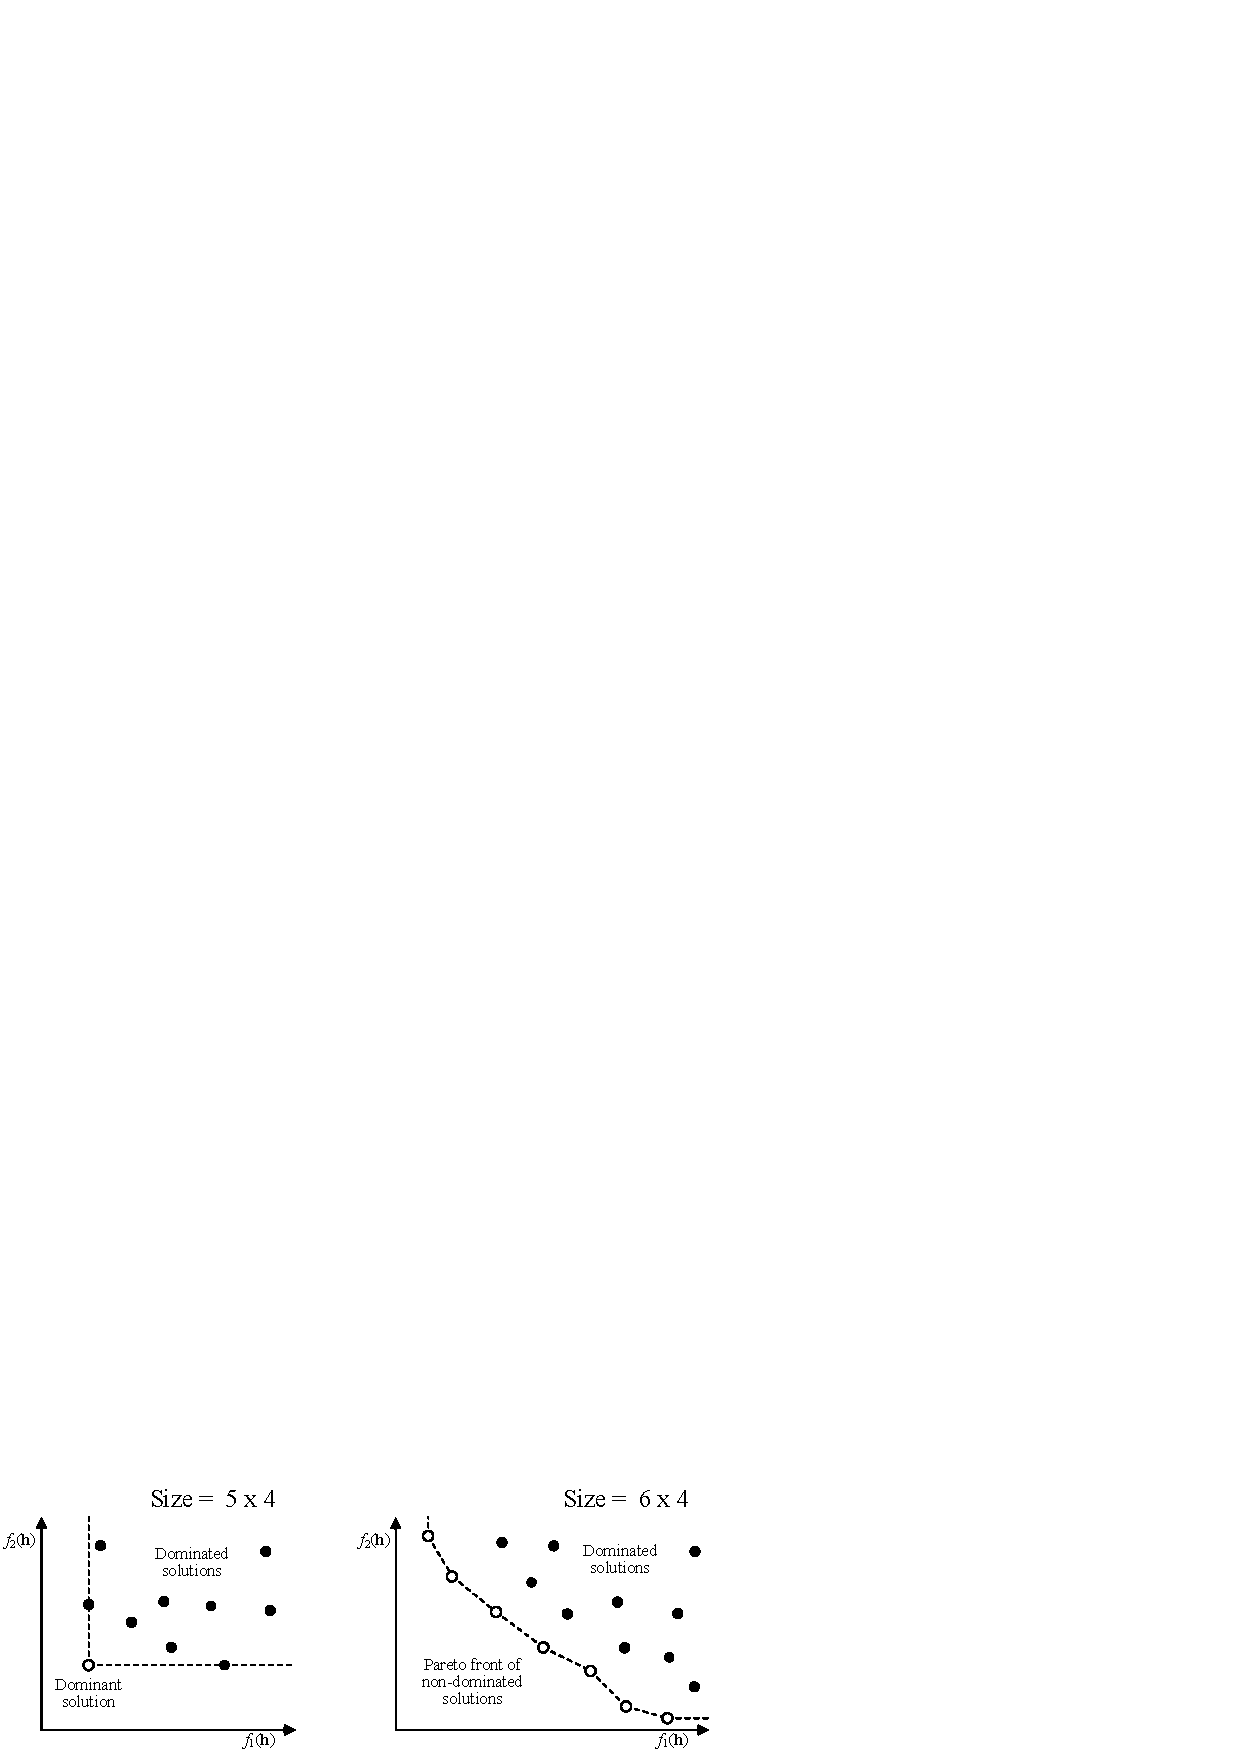
\includegraphics
  						 [height=4cm, viewport=0cm 0cm 5cm 4cm, clip]{c3_fig4}
  						 \label{fig:c3_dominance} }
 	\quad \quad
	\subfloat[Pareto front]{ 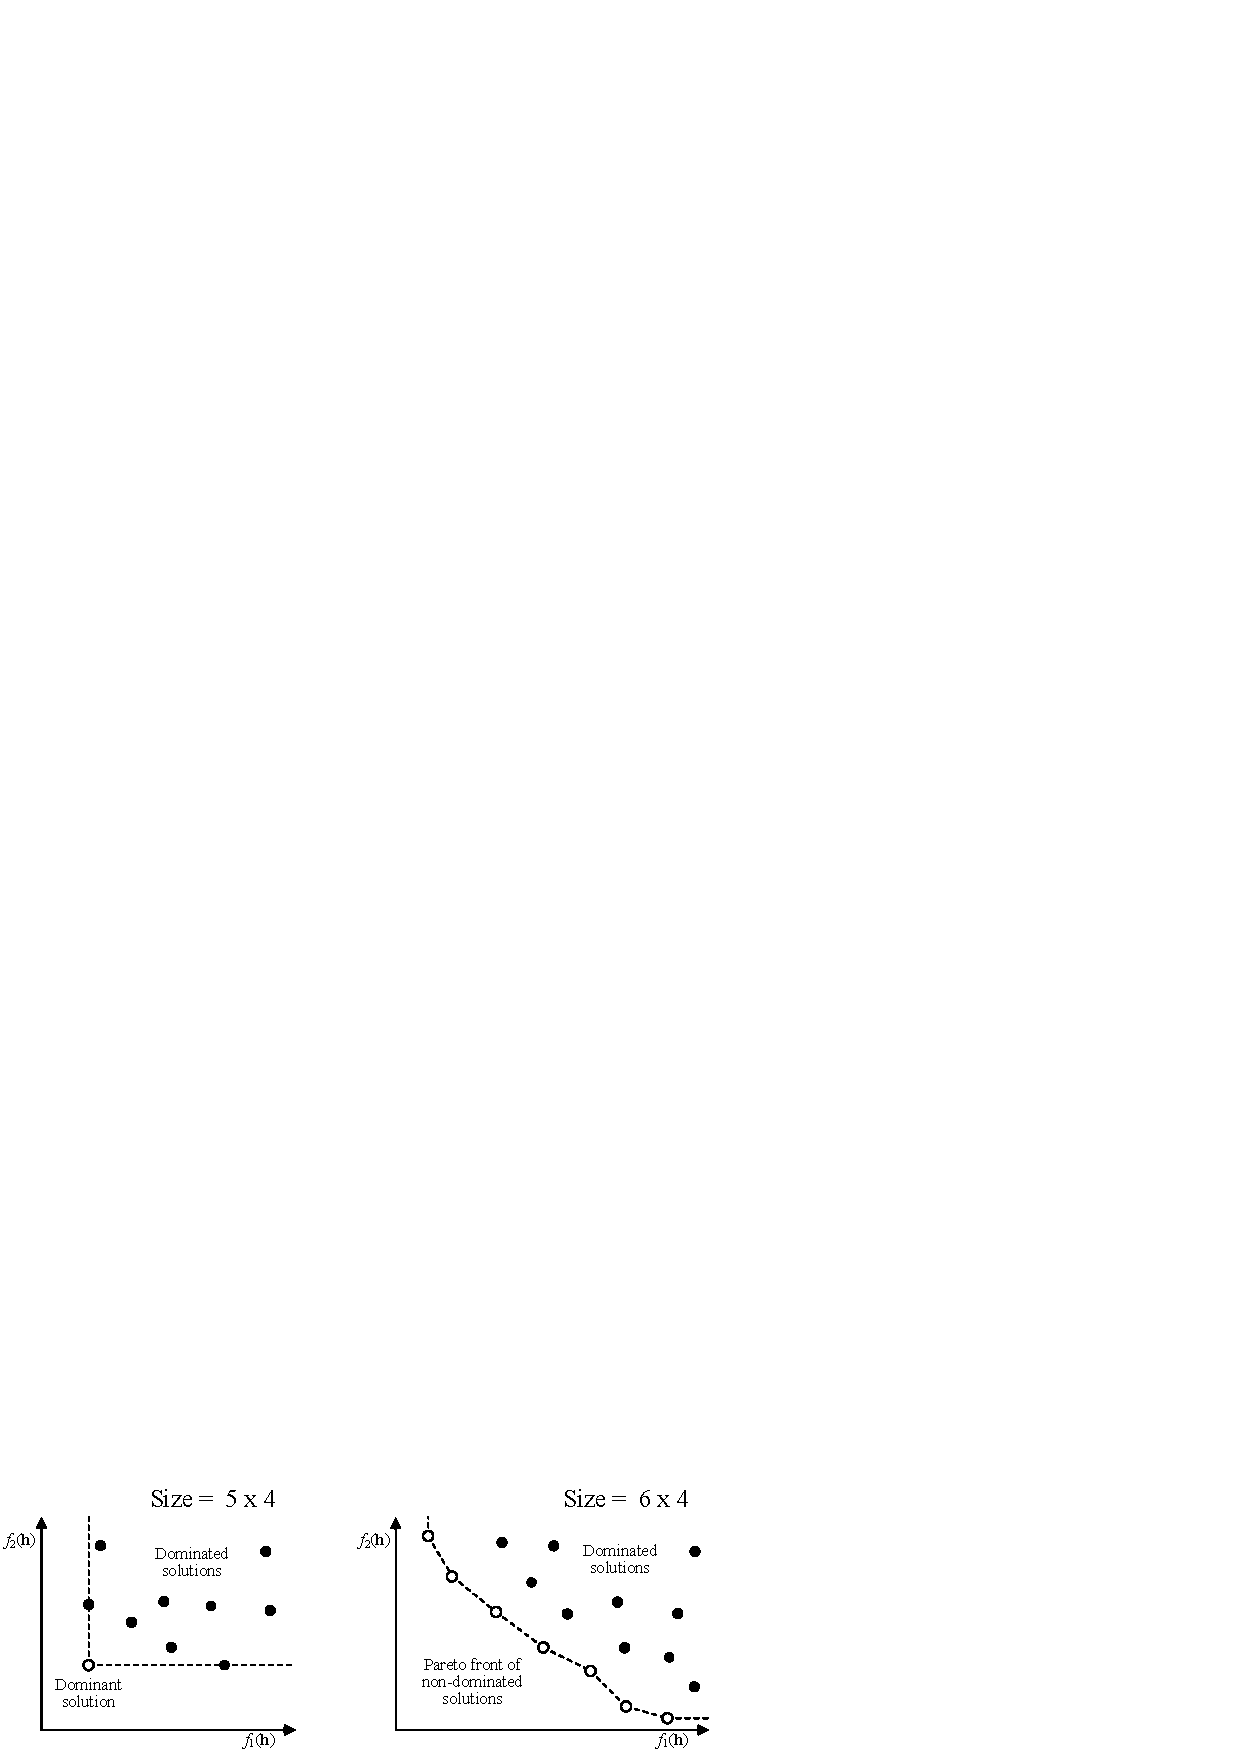
\includegraphics
  						 [height=4cm, viewport=6cm 0cm 12cm 4cm, clip]{c3_fig4}
  						 \label{fig:c3_parFront} } }
  \caption{Notion of dominance (\ref{fig:c3_dominance}) and Pareto optimal front (\ref{fig:c3_parFront}) for a MOO (minimization) problem in the objective space defined by two objectives $f_1(\mathbf{h})$ and $f_2(\mathbf{h})$}
	\label{fig:c3_pareto}
\end{figure*}
%--------------------------------- \Dominance ---------------------------------%

When adapting classifiers during incremental learning, another goal of the optimization algorithm is to seek hyperparameter values that generate a diversified pool of FAM networks among which ensembles can be selected.
As illustrated in Figure \ref{fig:c3_custom} with a simple MOO problem, the optimization process should provide accurate solutions with different network structural complexities.
This results in ensembles with good generalization capabilities, but with a possibility of limiting overall computational cost.

%---------------------------- Pareto front location ---------------------------%
\begin{figure*}[!t]
  \centering
  \fbox{\begin{minipage}{0.97\linewidth} \centering 
		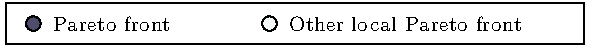
\includegraphics[width=0.68\linewidth]{c3_fig5_leg} \\
		\subfloat[Search space for $f_1(\textbf{\textbf{h}})$]{
		  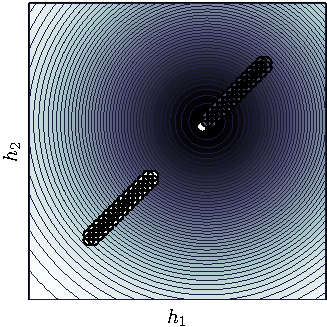
\includegraphics[width=0.30\linewidth]{c3_fig5a} } \quad
		\subfloat[Search space for $f_2(\textbf{\textbf{h}})$]{   		
			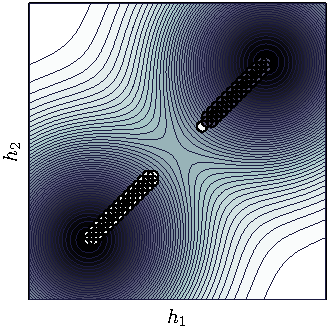
\includegraphics[width=0.30\linewidth]{c3_fig5b} } \quad
		\subfloat[Objective space]{ \label{fig:c3_pf}  		
			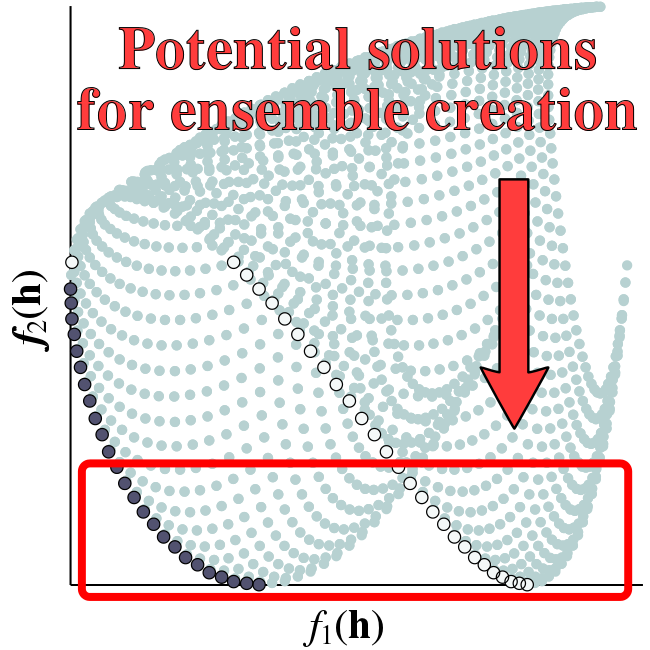
\includegraphics[width=0.30\linewidth]{c3_fig5c} }\\

\vspace{5pt}
\textbf{At $t=t+1$, after a change in $f_2(\textbf{\textbf{h}})$ only} \\

		\subfloat[Search space for $f_1(\textbf{\textbf{h}})$]{
		  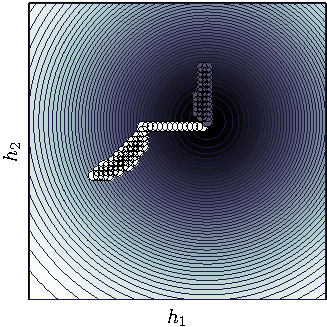
\includegraphics[width=0.30\linewidth]{c3_fig5d} } \quad
		\subfloat[Search space for $f_2(\textbf{\textbf{h}})$]{ \label{fig:c3_f2}   		
			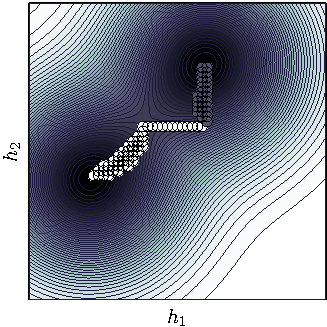
\includegraphics[width=0.30\linewidth]{c3_fig5e} } \quad
		\subfloat[Objective space]{ \label{fig:c3_pf2}  		
			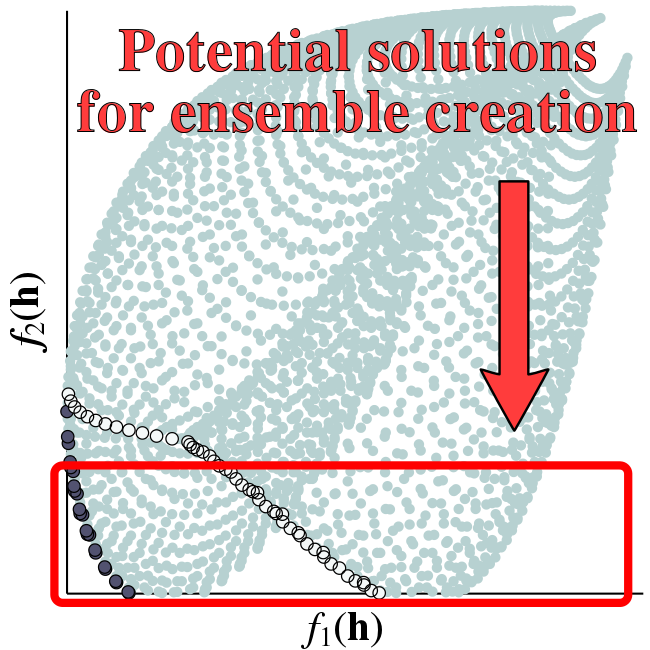
\includegraphics[width=0.30\linewidth]{c3_fig5f} }
  \end{minipage} }
  \caption{Position of local Pareto fronts in both search spaces and the objective space.
Obtained with a grid, true optimal solutions are illustrated by the dark circles and other locally Pareto-optimal solutions with light circles.
While the goal in a MOO is to find the optimal Pareto front (dark circles), another goal of the AMCS ADNPSO module is to search both search spaces to find solutions that are suitable for classifiers ensembles.
For instance, if at a time $t$, $f_1(\textbf{h})$ and $f_2(\textbf{h})$ respectively correspond to $f_s(\textbf{h},t)$ and $f_e(\textbf{h},t)$, these would be solutions in the red rectangle in Figures \ref{fig:c3_pf} and \ref{fig:c3_pf2} (with low generalization error and for a wide range of FAM network $F_2$ sizes).
Even if, at a time $t=t+1$, change occurs for only one objective function (Figure \ref{fig:c3_f2}), the entire objective space is affected and the problem must be considered dynamic}
	\label{fig:c3_custom}
\end{figure*}
%--------------------------- /Pareto front location ---------------------------%

In this particular case, the optimization algorithm also tackles a dynamic optimization problem by considering several objectives, and yield classifiers that correspond to vectors \textbf{h} that are not necessarily Pareto optimal (see Figure \ref{fig:c3_custom}).
Classical DPSO algorithms as well suited as MOO algorithms, such as Non-sorted genetic algorithm (NSGA) (\cite{deb02}), strength Pareto evolutionary algorithm (SPEA) (\cite{zitzler99}), multi-objective PSO (MOPSO) (\cite{coello04}), etc.
The only other approaches in literature aimed at generating and evolving a diverse population of FAM networks in term of structural complexity, yet contained non-dominated alternatives are presented in (\cite{granger10, li10}).
In \cite{granger10}, a MOPSO learning strategy is used to train FAM networks according both error rate and network size.
Although this strategy seeks to maintain phenotype diversity in the objective space, results showed that using MOPSO and a global Pareto-optimality criteria limits the number of non-dominated classifiers stored in the archive.
To circumvent this issue, a mimetic archive was instead used in \cite{li10} to prune $F_2$ nodes and categorize FAM networks in subpopulations that are independently evolved with a genetic algorithm.
With this method, FAM networks need to be pruned to maintain phenotype diversity, which is not the case in this chapter.


%------------------------------------------------------------------------------%
%------------------------------------------------------------------------------%
%------------------------------------------------------------------------------%
\section{Evolution of incremental learning ensembles}
\label{sec:c3_algo}

This chapter seeks to address challenges related to the design of robust AMCSs for video face recognition applications, where facial models are designed and updated over time, as new reference data becomes available.
An ADNPSO incremental learning strategy -- integrating an aggregated dynamical niching particle swarm optimization (ADNPSO) algorithm and a specialized archive -- is proposed to evolve heterogeneous classifier ensembles in response to new reference data.
Each particle in the optimization environment corresponds to a FAM network in the classification environment, and the ADNPSO incremental learning strategy evolves a swarm of classifiers such that both FAM generalization error rate and network size are minimized.

Particles are guided by the ADNPSO algorithm.
As with the DNPSO algorithm (\cite{nickabadi08_1}), the ADNPSO algorithm is also able to detect and track many local optima in a type III dynamic optimization environment.
In addition, it exploits several objective functions while maintaining genotype diversity in the search spaces, in particular around local optima.
However, unlike existing multi-objective optimization (MOO) algorithms (such as NSGA, MOEA, MOPSO, etc.), optimization does not rely on the objective space --
it exploits information available in the search space to determine fitness values and future search directions for each solution.
This results in an optimization algorithm that is influenced by different objectives.
It is aimed at generating pools of classifiers with high \emph{genotype} and \emph{phenotype} \emph{diversity}, rather than purely solving a MOO problem that provides the optimal Pareto front.
It does so by (1) maintaining diversity of solutions around the local optima in each search space, and (2) adjusting the position of each solution according to the different objective functions, to allow converging toward different local Pareto fronts.

Since particles are constantly moving with certain randomness and at great speed, a specialized archive of solutions divides the objective space according to FAM network structural complexity (\emph{i.e.}, $F_2$ layer size), and for each division, it captures non-dominated solutions locally along with their associated networks.
This effectively maintains a pool of classifiers with high phenotype diversity.
From this pool, a greedy search algorithm selects an ensemble of classifiers within the archive on the basis of accuracy, and \emph{both} genotype and phenotype diversity.

The DPSO-based incremental learning strategy developed in (\cite{connolly11}) has been modified to evolve heterogeneous ensembles in a MOO framework.
In particular, the ADNPSO strategy differs from previous research (1) in the way  networks are associated with each particle, (2) in the definition of the initial FAM network conditions used to estimate fitness, and (3) in the addition of a specialized archive to store solutions.

This rest of this section provides additional details on the news ADNPSO strategy, including the ADNPSO algorithm, specialized archive to store locally non-dominant solutions according to complexity, and learning strategy used to integrated those components to the AMCS.

%------------------------------------------------------------------------------%
%------------------------------------------------------------------------------%
\subsection{ADNPSO incremental learning strategy}
\label{sec:c3_strategy}

An ADNPSO incremental learning strategy (Algorithm \ref{alg:c3_dmopso}) is proposed to evolve FAM networks according multiple objectives and accumulate a pool of FAM networks in the specialized archive (see Section \ref{sec:c3_mimetism}), and ensemble selection.
During incremental learning of a data block $D_t$, FAM hyperparameters, parameters and architecture are cojointly optimized such that the generalization error rate and network size are minimized.
Based on the hypothesis that maintaining diversity among particles in the optimization environment implicitly generates diversity among classifiers in the classification environment (\cite{connolly11}), properties of the ADNPSO algorithm is used to evolve a diversified heterogeneous ensembles of FAM networks over time.

At a time $t$, and for each particle $n$, the current particle position is noted $\textbf{h}_n$, along with its personal best values on each objective function $o$, $\textbf{h}^*_{n,o}$.
The values estimated on the objective functions and the best position of each particle are respectively noted $f_o(\textbf{h}_n,t)$ and $f_o(\textbf{h}^*_{n,o},t)$. 
For $O$ objectives, and the ADNPSO algorithm presented in Section \ref{sec:c3_adnpso} that uses $N$ particles, a total of $(O+2)N$ FAM networks are required.
For each particle $n$, the AMCS stores:
\begin{enumerate}
	\item $O$ networks $\textit{FAM}_{n,o}$ associated with $\textbf{h}^*_{n,o}$ (particle $n$ personal best position on objective function $o$),
	\item the network $\textit{FAM}_n^\text{start}$ associated to the current position of the each particle $n$ after convergence of the optimization process at time $t-1$, and 
	\item the network $\textit{FAM}_n^\text{est}$ obtained after learning $D_t$ with current position of particle $n$ (noted $\textbf{h}_n$).
\end{enumerate}
While $\textit{FAM}_n^\text{start}$ represents the state of the particle before learning $D_t$, $\textit{FAM}_n^\text{est}$ is the state of the same particle after having explored a position in the search space, and it is used for fitness estimation.

%-------------- Algorithm : ADNPSO incremental learning algorithm -------------%
\begin{algorithm}[!b]
	\caption{ADNPSO incremental learning strategy (continued next page)}
	\label{alg:c3_dmopso}
 	\fbox{\begin{minipage}{0.97\linewidth}\centering
	\begin{algorithmic}[1]
		\Require An AMCS and new data sets $D_t$ for learning.
		\Ensure  A pool of accurate FAM networks with different complexity 
					   phenotype diversity.
						
		\Statex\vspace{6pt} \textbf{Initialization:}\vspace{3pt}
		\State  $\bullet$ Set the swarm and archive parameters,
		\Statex	$\bullet$ Initialize all $(O+2)N$ networks: 
					 					  $\textit{FAM}_{n,o}$, $\textit{FAM}_n^\text{start}$, and 
					 					  $\textit{FAM}_n^\text{start}$, 
		\Statex $\bullet$ Randomly initialize particles positions and velocities, and set ADNPSO iteration counter at $\tau=0$.
					 																									\label{l:c3_init}
		%-- For each learning block
		\Statex\vspace{9pt} \textbf{Upon reception of a new data block $D_t$, the following incremental process is initiated:}\vspace{3pt}
			%-- Personal best update
			\Statex\textit{$\bullet$ \underline{Update the fitness of networks associated to the personal best positions:}}\vspace{3pt}
			\For{ each particle $n$, where $ 1 \leq n \leq N$ }
				\For{ each objectives $o$, where $1\leq o\leq O$ }	\label{l:c3_pUpdate}
					\State Train and validate $\textit{FAM}_{n,o}$ with $D_t^\text{t}$
								 and $D_t^\text{v}$ respectively.
					\State Estimate $f_o(\textbf{h}^*_{n,o}, t)$ using $D_t^\text{f}$.
				\EndFor
			\EndFor      \label{l:c3_pUpdateEnd}

			\Statex\vspace{6pt}\textit{$\bullet$ \underline{Update the specialized archive:}}\vspace{3pt}
			\State Update the accuracy of each solution in the archive. 
																													\label{l:c3_arcUpdate}
			\State Remove locally dominated solutions form the archive.
																													\label{l:c3_remove}
			\For{ each particle $n$, where $ 1 \leq n \leq N$ }
				\For{ each objectives $o$, where $1\leq o\leq O$ }
					\State Categorize $\textit{FAM}_{n,o}$.
					\If {$\textit{FAM}_{n,o}$ is a non-dominated solution 
								for its network size domain}							
						\State Add the solution to the specialized archive.
						\State Remove solutions in the archive that are locally dominated 
									 by $\textit{FAM}_{n,o}$.
					\EndIf					
				\EndFor
			\EndFor                                          \label{l:c3_arcUpdateEnd}
%-- Breaking that algorithm in two			
	\algstore{somename}	\end{algorithmic} 	\end{minipage} } \end{algorithm}
	\begin{algorithm}[t]
%	\caption{ADNPSO incremental learning strategy (part 2/2).}
 	\fbox{\begin{minipage}{0.97\linewidth}\centering
	\begin{algorithmic}[1] \algrestore{somename}
%-- /Breaking that algorithm in two			
			
			%-- Loop iterations
			\Statex\vspace{6pt}\textit{$\bullet$ \underline{Optimization process:}}\vspace{3pt}
			\While{the optimization algorithm does not reach its stopping condition}																												    \label{l:c3_opt}
				\State Update particle positions according to the ADNPSO algorithm
				       (Equation \ref{eq:c3_adnpso}). \label{l:c3_newPos}
				
				\Statex\vspace{6pt}\hspace{15pt}\textit{--- Estimate fitness and update
							 personal best positions:}\vspace{3pt}
				\For{each particle $n$, where $ 1 \leq n \leq N$}
					\State $\textit{FAM}_n^\text{est}$ $\leftarrow$   
								 $\textit{FAM}_n^\text{start}$							\label{l:c3_start}
					\State Train $\textit{FAM}_n^\text{est}$ with validation using
								 $D_t^\text{t}$ and $D_t^\text{v}$.					\label{l:c3_trn}
					\State Estimate $f_o(\textbf{h}_n(\tau),t)$ of each objective using
								 $D_t^\text{f}$.														\label{l:c3_est}
					\For{each objective $o$, where $1\leq o\leq O$}		\label{l:c3_pAdjust}
						\If{ $f_o(\textbf{h}_n(\tau),t) < f_o(\textbf{h}^*_{n,o},t)$ }
							\State \{\ $\textbf{h}^*_{n,o}$, $\textit{FAM}_{n,o}$,
											 $f_o(\textbf{h}^*_{n,o},t)$\ \} $\leftarrow$ 
										 \{\ $\textbf{h}_n(\tau)$, $\textit{FAM}_n^\text{est}$,
										   $f_o(\textbf{h}_n(\tau),t)$\ \}.			
						\EndIf
					\EndFor	
					
					\Statex\vspace{6pt}\hspace{30pt}\textit{- Update the specialized
								 archive:}\vspace{3pt}
					\State Categorize $\textit{FAM}_n^\text{est}$			\label{l:c3_arcCur}
					\If{$\textit{FAM}_n^\text{est}$ is a non-dominated solution 
							for its network size domain}
						\State Add the solution to the specialized archive
						\State Remove solutions in the archive that are locally dominated 
									 by $\textit{FAM}_n^\text{est}$.
					\EndIf																				\label{l:c3_arcCurEnd}

				\EndFor																					\label{l:c3_pAdjustEnd}

				\State Increment iterations: $\tau = \tau + 1$.    \label{l:c3_itUpdate}
			\EndWhile 																						\label{l:c3_endOpt}

			\Statex\vspace{6pt}\textit{$\bullet$ \underline{Define initial conditions for fitness estimation with $D_{t+1}$:}}\vspace{3pt}
			\For{ each particle $n$, where $ 1 \leq n \leq N$ }		\label{l:c3_sUpdate}
				\State $\textit{FAM}_n^\text{start}$ $\leftarrow$
							 $\textit{FAM}_n^\text{est}$.
			\EndFor   \label{l:c3_sUpdateEnd}
	\end{algorithmic}
		\end{minipage} }

\end{algorithm}
%------------------------------------------------------------------------------%

Particle positions are then randomly initialized within their allowed range.
When a new $D_t$ becomes available, the optimization process begins.
Using the new data and for all objectives $o$, fitness associated with the best position of each particle ($f_o(\textbf{h}^*_{n,o},t)$) is updated along with each network $\textit{FAM}_{n,o}$ (lines \ref{l:c3_pUpdate}--\ref{l:c3_pUpdateEnd}).
The archive is then updated (lines \ref{l:c3_arcUpdate}--\ref{l:c3_arcUpdateEnd}).
Accuracy of the solutions in the archive are also updated and checked for non-dominance.
The archive is then filled accordingly with the networks $\textit{FAM}_{n,o}$.

During the initialization process (line \ref{l:c3_init}), the swarm and all FAM networks are initialized.
Particle positions are randomly initialized within their allowed range.
When a new $D_t$ becomes available, the optimization process begins.

Networks associated with the best position of each particle ($\textit{FAM}_{n,o}$) are incrementally updated using the new data, along with their fitnesses $f_o(\textbf{h}^*_{n,o},t)$ (lines \ref{l:c3_pUpdate}--\ref{l:c3_pUpdateEnd}).
Network in the archive and their fitnesses are also updated in the same manner (lines \ref{l:c3_arcUpdate}--\ref{l:c3_arcUpdateEnd}).
Since accuracy corresponds to dynamic optimization problem, Algorithm \ref{alg:c3_dmopso} verifies if solutions then still respect the non-dominant criteria of the specialized archive.
Afterward, the specialized archive is filled accordingly using the networks $\textit{FAM}_{n,o}$.

Optimization then continues were it previously ended until the ADNPSO algorithm converges (lines \ref{l:c3_opt}--\ref{l:c3_endOpt}).
During this process, the ADNPSO algorithm explores the search spaces (line \ref{l:c3_newPos}).
It then copy $\textit{FAM}_n^\text{start}$ to redefines the state of $\textit{FAM}_\text{est}$ prior learning at a time $t$, trains the latter using $\textbf{h}_n$, and estimates its fitness (lines \ref{l:c3_start}--\ref{l:c3_est}).
For each objective $o$, the best position ($\textbf{h}^*_{n,o}$) and its corresponding fitness ($f_o(\textbf{h}^*_{n,o},t)$) and network ($\textit{FAM}_{n,o}$) are updated if necessary (lines \ref{l:c3_pAdjust}--\ref{l:c3_pAdjustEnd}).
In the cases of equality between $f_o(\textbf{h}_n,t)$ and $f_o(\textbf{h}^*_{n,o},t)$, the network that requires the least resources ($F_2$ nodes) is used.
Each time fitness is estimated at a particle's current position, $\textit{FAM}_\text{est}$ is categorize according its network size and added to the archive if it is non-dominated for its $F_2$ size domain (lines \ref{l:c3_arcCur}--\ref{l:c3_arcCurEnd}). 
Finally, the iteration counter is incremented (line \ref{l:c3_itUpdate}).

Once optimization converges, networks corresponding to the last position evaluated of every particle ($\textit{FAM}_n^\text{est}$) are stored in $\textit{FAM}_n^\text{start}$ (lines \ref{l:c3_sUpdate}--\ref{l:c3_sUpdateEnd}).
These networks will thus define the swarm's state prior learning data block $D_{t+1}$.

During this Algorithm \ref{alg:c3_dmopso} each time fitness is estimated, FAM networks are trained using the training data set $D_t^\text{t}$ under five different random pattern presentation orders to minimize the impact of pattern presentation order at a time $t$.
Since the primary objective is accuracy, $\textit{FAM}_n^\text{est}$ is the network that yields the lowest error rate and the fitness for each objective is defined according the latter.

%------------------------------------------------------------------------------%
%------------------------------------------------------------------------------%
\subsection{Aggregated dynamical niching PSO}
\label{sec:c3_adnpso}

Particle swarm optimization (PSO) is a population-based stochastic optimization technique that is inspired by social behavior of bird flocking or fish schooling.
By associating a classifier to each particles, PSO is a powerful tool to cojointly optimize swarms of classifiers hyperparameters, parameters, and architecture.
With PSO, each particle corresponds to a single solution in the optimization space, and the population of particles is called a swarm.
Unlike evolutionary algorithms (such as genetic algorithms), each particle always stores its best position and the best position of its surrounding.
In a mono-objective problem and at a discrete iteration $\tau$, particles move through the hyperparameter space and change their positions $\textbf{h}(\tau)$ under the guidance of $\Phi$ sources of influence (\cite{kennedy07}):
\begin{equation}  \label{sgen}
		\textbf{h}\left(\tau+1\right) = \textbf{h}(\tau) \ +\ w_0 \ 
																		( \textbf{h}(\tau) - \textbf{h}(\tau-1) )
           \ +\ \displaystyle\sum_{\phi=1}^\Phi r_\phi \ 
             w_\phi \ ( \textbf{h}_\phi - \textbf{h}(\tau) ),
\end{equation}
where $\phi$ is the index of a source of influence, $r_\phi$ a random number, $w_0$ an inertia weight, and $w_\phi$ the weights indicating the importance each influence.
With this formalism, each particle (1) begins at its current location, (2) continues moving in the same direction it was going according to an inertia weight $w_0$, and (3) is attracted by each source of influence according to a random weight $w_\phi$.

PSO algorithms evolve the swarm according to a \emph{social influence} (\emph{i.e.}, their neighborhood previous search experience) and a \emph{cognitive influence} (\emph{i.e.}, their own previous search experience).
For instance, with a canonical PSO algorithm, Equation \ref{eq:c3_pso} becomes
\begin{equation}  \label{eq:c3_pso}
	\begin{split}
		\textbf{h}\left(\tau+1\right) = & \textbf{h}(\tau) \ +\ 
						w_0( \textbf{h}(\tau) - \textbf{h}(\tau-1) ) \\
        & +\ r_1 w_1( \textbf{h}_\text{social influence} - \textbf{h}(\tau) ) \\
        & +\ r_2 w_2( \textbf{h}_\text{cognitive influence} - \textbf{h}(\tau)).
	\end{split}
\end{equation}

Although originally developed for static optimization problems, PSO formalism has been adapted to suit the nature of the optimization problem at hand.
For instance, it has been adapted for dynamic optimization problems by adding mechanisms to (1) modify the social influence to maintain diversity in the optimization space and detect several optima, (2) detect changes in the objective function by using the memory of each particle, and (3) adapt the memory of its population if change occurs in the optimization environment.
The latest particle swarm optimization algorithms developed to insure diversity in the swarm are presented in \cite{du08, li06, nickabadi08_2, ozcan07}.
Change detection and memory adjustment mechanisms for DPSO are presented in \cite{blackwell04, carlisle02, hu02, wang07}.

PSO algorithms have also been adapted for MOO in three ways by (1) defining social and cognitive influences according to a fitness function based on the notion of Pareto-dominance (see Figure \ref{fig:c3_dominance}), (2) storing non-dominated solutions in an archive, and (3) managing phenotype diversity in the objective space.
A review of multi-objective particle swarm optimization (MOPSO) algorithms is given in \cite{reyes06}.
Most of these approaches uses a global best topology and focus on moving particles according to the Pareto front rather than local optima in the search space.
Under the hypothesis that many solutions will be stored in an archive, they also use classic archive that considers only global Pareto-optimality.

To generate a pool of classifiers, ADNPSO uses the same approach as mono-objective optimization algorithms, and defines influences in the different search spaces, with the objective functions.
This is achieved by reformulating the general PSO definition (Equation \ref{eq:c3_pso}) according two objectives: error rate ($f_e(\mathbf{h},t)$) and network $F_2$ size ($f_s(\mathbf{h},t)$) of each FAM network.
Each particle will then move according to a cognitive and social influence for both objectives (see Figure \ref{fig:c3_influences}), formally defined by:
\begin{equation}
	\begin{split}
		\textbf{h}\left(\tau+1\right) = \  
		  & \textbf{h}(\tau) + w_0\ ( \textbf{h}(\tau) - \textbf{h}(\tau-1) )\\
		    & + r_1\ w_1\
				    ( \textbf{h}_\text{social influence, error rate}    - 		
				    	\textbf{h}(\tau) )\\
				& + r_2\ w_2\ 
				    ( \textbf{h}_\text{cognitive influence, error rate} - 	
				    	\textbf{h}(\tau) )\\  				      
				& + r_3\ w_3\ 
				    ( \textbf{h}_\text{social influence, network size}    - 
				    	\textbf{h}(\tau) )\\
				& + r_4\ w_4\ 
				    ( \textbf{h}_\text{cognitive influence, network size} - 
				      \textbf{h}(\tau) ),
	\end{split}
	\label{eq:c3_adnpso}
\end{equation}
As previously showed in Figure \ref{fig:c3_custom}, the rational behind this approach is that when several local optima are present in different search spaces, non-dominated solutions tend to be located in regions between local optima of the different objectives.
By adjusting the weights $w_\phi$, a swarm may be biased according to one objectives or even divided in three subpopulations : (1) one that specializes in accuracy ($w_1$ and $w_2$ $>$ $w_3$ and $w_4$), (2) one that specializes in complexity ($w_1$ and $w_2$ $<$ $w_3$ and $w_4$), and (3) a generalist subpopulation that put both objectives on equal footing ($w_1=w_2=w_3=w_4$).

Social influences of both objectives are managed by creating subswarms that adapt the DNPSO local neighborhood topology (\cite{nickabadi08_1}) to multiple objectives.
While DNPSO creates subswarms dynamically around the \emph{current position} of local best particles (\emph{i.e.}, particles with a personal best position that has the best fitness in their neighborhood), ADNPSO uses the memory of these local best particles.
Social influences are then \emph{personal best position} of local best particles computed independently for both objectives.
As shown in Figure \ref{fig:c3_influences}, by limiting the size of each subswarm, particles can be excluded of these subswarms for none, one, or both objectives.
For the objective that was excluded, a particle is said to be ``free'' and its social influence is removed by setting the weights $w_1=0$ and/or $w_3=0$ when computing Equation \ref{eq:c3_adnpso} (depending for which objective(s) the particle is ``free'').
This way, a poor compromise can be avoided, and conflicting influences can then be managed simply by limiting the maximal size of each subswarm.

The DNPSO local neighborhood topology offer many ways to insure particle diversity in the search space (\cite{nickabadi08_2}).
It is also adapted to also maintain cognitive (\emph{i.e.}, personal best) diversity among particles within each subswarm.
The ADNPSO algorithm defines a distance $\Delta$ around local best positions of each objectives.
Every time a particle moves with the distance $\Delta$ from the detected local optima of one objective, the personal best value of that particle is erased (\emph{i.e.}, ``loses its memory'').
It then moves only according the other objectives by setting designated weights to 0.
Since MOO problems generally have conflicting objectives, this results in particles that move away from the local optima when they are within the distance $\Delta$ from each other.

%--------------------------------- Influences ---------------------------------%
\begin{figure*}[t]
  \centering
	\fbox{
		\subfloat[Search space for $f_1(\textbf{h})$]{ \label{fig:c3_sub1}
		  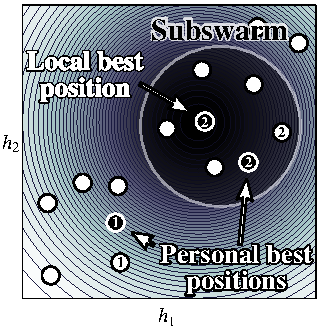
\includegraphics[width=0.3\linewidth]{c3_fig6a} }\quad
		\subfloat[Search space for $f_2(\textbf{h})$]{ \label{fig:c3_sub2}
			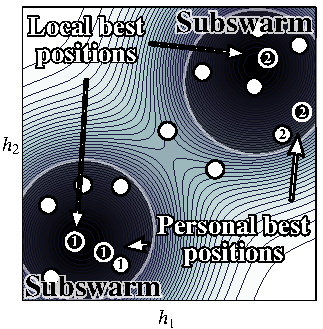
\includegraphics[width=0.3\linewidth]{c3_fig6b} }\quad
		\subfloat[Particle movements]{   		
			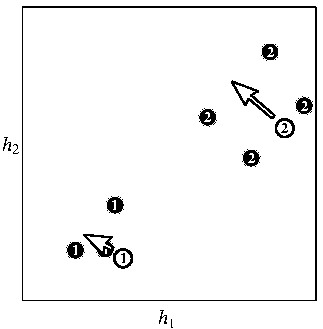
\includegraphics[width=0.3\linewidth]{c3_fig6c} } \label{fig:c3_inf3}
	}
  	\caption{An illustration of influences in the search spaces and resulting movements.
Given the same objective functions used in Figure \ref{fig:c3_custom}, two particles in a swarm (white circles), and their social and cognitive influences (black circles), let subswarms have a maximal size of 5 particles.
Both particles 1 and 2 have cognitive influences in both search spaces, yet particle 1 is not part of any subswarm for $f_1(\textbf{h})$. 
Unlike particle 2, it has no social influence for this objective and ADNPSO sets $w_1=0$ when computing its movement with Equation \ref{eq:c3_adnpso}}
	\label{fig:c3_influences}
\end{figure*}
%-------------------------------- /Influences ---------------------------------%

The computational cost of the ADNPSO algorithm depends on the time needed takes to create subswarms and to manage particle positions during the optimization process.
For each particle, it must (1) sort the rest of the swarm according to a distance metric to define the neighborhood, and (2) sort the neighbors by fitness to find the local best.
In contrast, as it is explained in Section \ref{sec:c3_strategy}, each time fitness is estimated, a FAM neural network must be trained and tested.
Since, managing the swarm with the ADNPSO algorithm requires a computational cost significantly lower than that necessary to update the fitness of the swarm, 
it should not be considered when applied to the AMCS.

%------------------------------------------------------------------------------%
%------------------------------------------------------------------------------%
\subsection{Specialized archive and ensemble selection}
\label{sec:c3_mimetism}

A specialized archive is introduced in the AMCS framework to store a pool of classifier such phenotype diversity in the objective space is maintained according to FAM network size, and as framework for ensemble selection.
In the ADNPSO incremental learning strategy (Section \ref{sec:c3_strategy}), the archive regroups FAM networks associated with each solution found in the search space according to their structural complexity (\emph{i.e.}, number of $F_2$ nodes) and stores them in to create a pool of classifiers among which ensembles can be selected.

Since the AMCS is applied to an ill-defined pattern recognition problem, where a limited amount of reference data is used for system design, both objectives are discrete functions, and the error rate is prone to over fitting.
In this context, the specialized archive is used to (1) insure phenotype diversity in the objective space according to FAM network size, and (2) as framework for ensemble selection.
As shown in Figure \ref{fig:c3_mimetism}, the archive categorizes FAM networks associated with each solution found in the search space according to their $F_2$ layer size and stores them to create a pool of classifiers among which ensembles can be selected.
Although, this imply keeping dominated solutions in the objective space for a MOO formulation, using a specialized archive ensures storing classifiers with a wide phenotype diversity in structural complexity.

When a new block $D_t$ of reference samples becomes available at a time $t$, the swarm evolves in the search spaces and the performance of each network is re-evaluated using a mixture of new data and old data (in the LTM).
However, since no further training occurs once they are stored in the archive, the size of the FAM networks in the archive never changes.
Compact classifiers obtained in earlier blocks may remain in the archive over time as new data is learned incrementally.

%----------------------------- Specialized archive ----------------------------%
\begin{figure*}[t]
  \centering
  \fbox{
		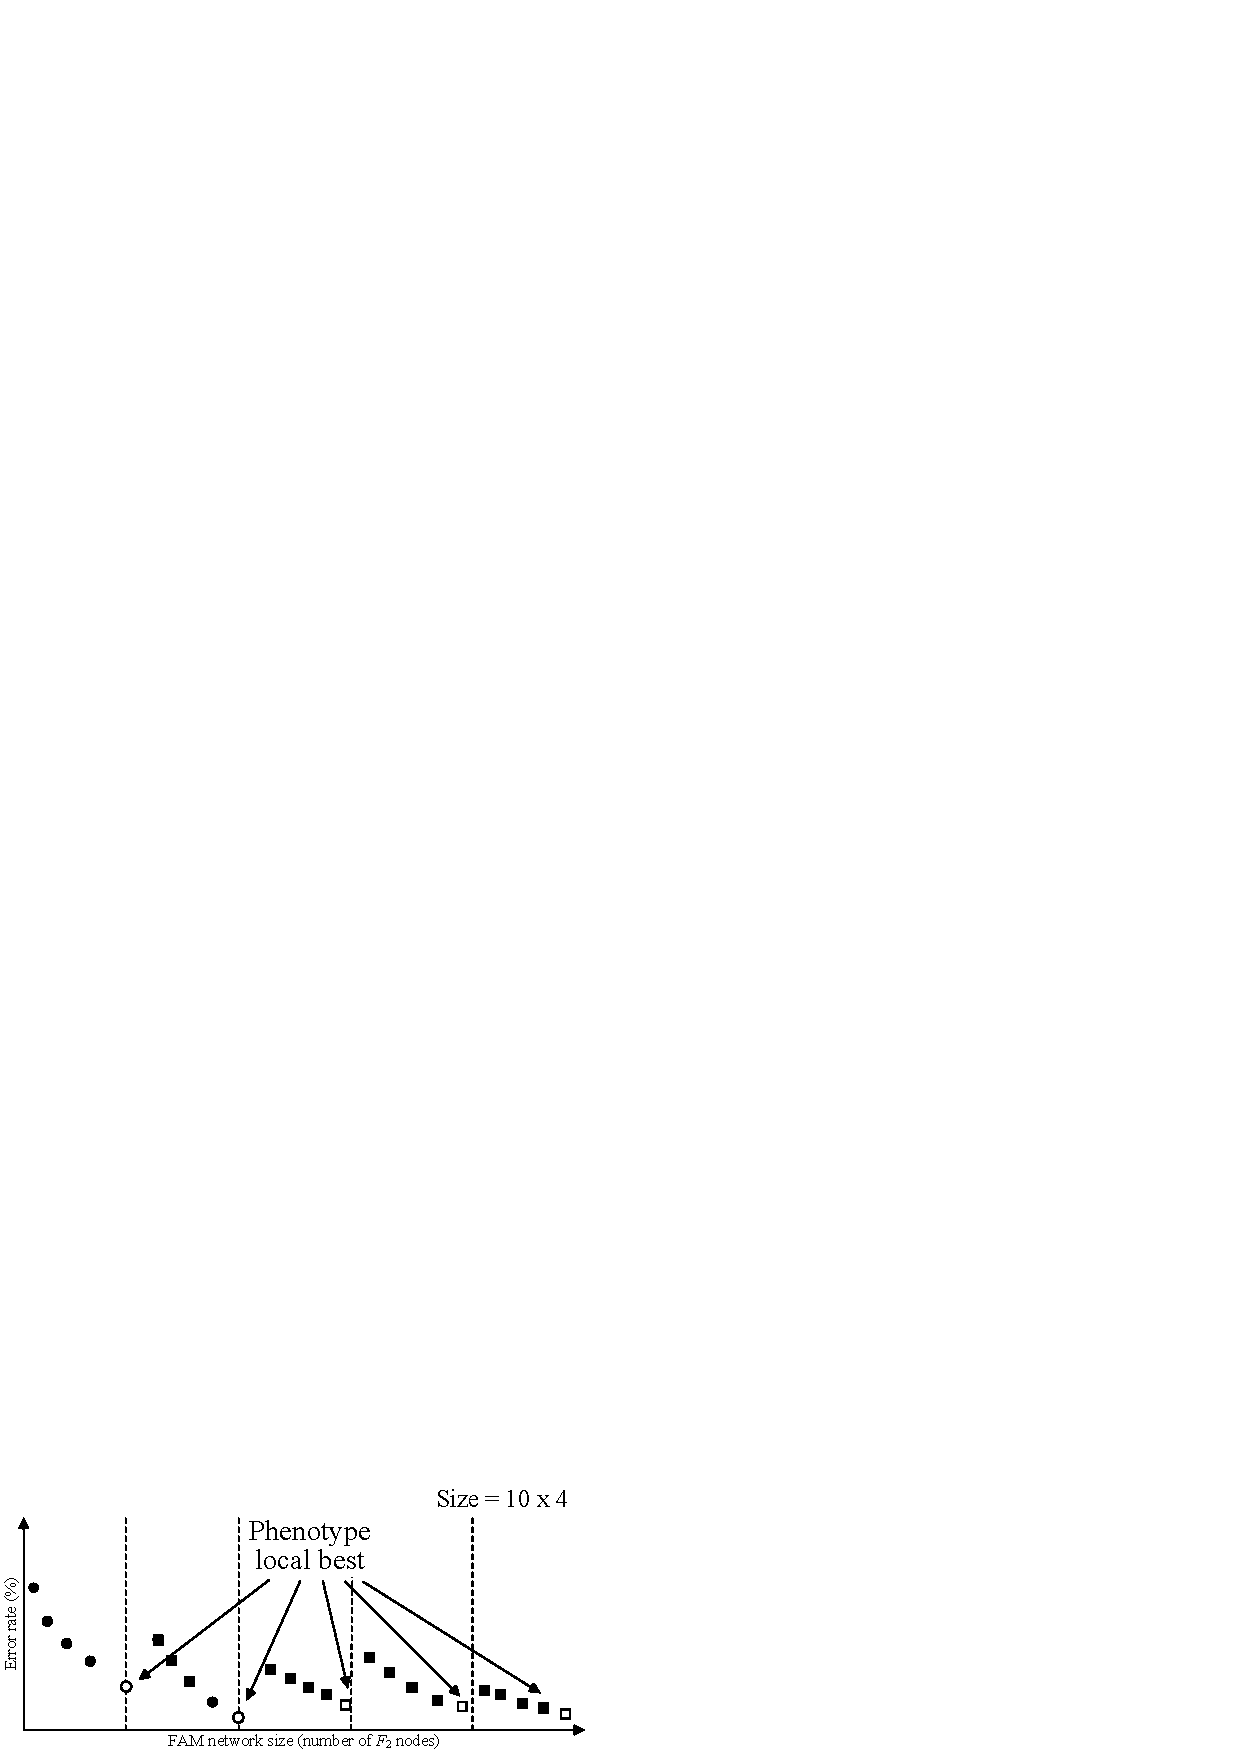
\includegraphics[width=0.70\linewidth, viewport = 0cm 0cm 10cm 4cm, clip]
										{c3_fig7} }
 	\caption{Illustration of the specialized archive of solutions in the objective space.
The FAM network size objective is segmented in different domains (or slices of complexity), where both Pareto-optimal (circles) and locally Pareto-optimal (squares) solutions are kept in the archive.
The local best are defined as the most accurate network of each size domain}
	\label{fig:c3_mimetism}
\end{figure*}
%---------------------------- /Specialized archive ----------------------------%

With the ADNPSO algorithm, a genotype local best topology is used to define neighborhoods and zones of influence for the different particles in the search space.
The same principle is applied in the objective space for ensemble selection.
The most accurate FAM of each network size domain are considered as phenotype local best solutions.
Classifiers are selected to create an initial ensemble that is completed with a second selection phase that uses a greedy search process (introduced in \cite{connolly11} to increase classifier diversity by maximizing their genotype diversity.
The result of the overall selection process is an ensemble with: 
\begin{enumerate}
	\item high phenotype diversity of FAM network sizes, where networks of different structural complexity are considered, even though the estimated generalization capabilities of the some networks are not necessarily the highest or Pareto-optimal, and 
	\item diversified classifiers in both feature and decision spaces 
			  (\cite{connolly11}).
\end{enumerate}

Unlike other approaches in the literature, the proposed AMCS does not consider time as a factor to add/remove a classifier from the ensemble.
It uses the notions of dominance and phenotype diversity.
If classifiers become obsolete in time due to a decrease in their accuracy, they will lose their dominant position and eventually be erased from the archive.
On the other hand, although they remain in the archive, solutions that do not increase ensemble diversity are never selected.

%------------------------------------------------------------------------------%
%------------------------------------------------------------------------------%
%------------------------------------------------------------------------------%
\section{Experimental methodology}
\label{sec:c3_methodology}

This chapter focuses on the appearance-based classification aspect of the face recognition system by replacing the classification module and biometric data base (in Figure \ref{fig:c3_faceRec}) by the proposed AMCS.
The rest of the system relies on classical algorithms.
%Segmentation is performed with the well known Viola-Jones algorithm included in the OpenCV C/C++ computer vision library.
%Moreover, tracking is assumed to be ideal so that continuous video sequences are composed of the detected ROIs.
As recognition is perform with an AMCS based on the FAM classifier, the responses for each successive ROI is a binary code (equals to ``1'' for the predicted class, and ``0''s for the others).
For a video sequence of a given length, the predicted class label $C_k$ is the one with the highest accumulated response obtained for each ROI (\emph{i.e.}, a majority vote between predictions for each individual ROI).

The rest of this section describes the procedure utilized to perform proof-of-concept experiments, including data bases, incremental learning scenarios, experimental protocol, and performance indicators.

%---------------------------- subsection : Database ---------------------------%
\subsection{Video data bases}
\label{sec:c3_db}

The first data base was collected by the Institute for Information Technology of the Canadian National Research Council (IIT-NRC) (\cite{gorodnichy05}).
It is composed of 22 video sequences captured from eleven individuals positioned in front of a computer.
For each individual, two color video sequences of about fifteen seconds are captured at a rate of 20 frames per seconds with an Intel web cam of a $160\times120$ resolution that was mounted on a computer monitor.
Of the two video sequences, one is dedicated to training and the other to testing.
They are taken under approximately the same illumination conditions, the same setup, almost the same background, and each face occupies between $1/4$ to $1/8$ of the image.
This data base contains a variety of challenging operational conditions such as motion blur, out of focus factor, facial orientation, facial expression, occlusion, and low resolution.
The number of ROIs detected varies from class to class, ranging from 40 to 190 for one video sequences.

The second video data base is called Motion of Body (MoBo), and was collected at Carnegie Mellon University under the HumanID project (\cite{gross02}).
Each video sequence shows one of 25 different individuals on a tread-mill so that they move their heads naturally to four different motion types when walking: slowly, fast, on an inclined surface, and while carrying an object.
Six Sony DXC 9000 cameras, with a resolution of a $640\times480$ pixels, are positioned at different locations around the individuals.
Only the video sequences with visible faces were kept: full frontal view and both sides with an angle of about $70^\circ$ with the full frontal view.

Segmentation is performed using the well known Viola-Jones algorithm included in the OpenCV C/C++ computer vision library.
In both cases, regions of interest (ROIs) produced are converted in gray scale and normalized to $24\times24$ images where the eyes are aligned horizontally, with a distance of 12 pixels between them.
Principal Component Analysis is then performed to reduce the number of features.
For the IIT-NRC data base, the 64 features with the greatest eigenvalues are extracted and vectorized into $\textbf{a} = \{a_1, a_2, ..., a_{64}\}$, where each feature $a_i \in [0,1]$ are normalized using the min-max technique.
Learning is done with ROIs extracted from the first series of video sequences (1527 ROIs for all individuals) while testing is done with ROIs extracted from the second series of video sequences (1585 ROIs for all individuals).
The ROIs obtained with the MoBo data base where processed with Local Binary Pattern and Principal Component Analysis to produce 32 features vectors, also normalized using the min-max technique.
ROIs from sequences for each type of walk and view are divided in two; the first half is used for learning and the second half, for testing.
This yields a total of 36374 learning patterns and 36227 test patterns.
In both cases, the number of features was fixed after error convergence with a 1NN classifier trained on the learning data bases and tested on the test data base.
Moreover, to insure that no false positive are present during training and testing, the ROIs have then been manually filtered.

%------------------------------------------------------------------------------%
\subsection{Incremental learning scenarios}
\label{sec:c3_scenario}

Prior to computer simulations, each video data set is divided in blocks of data $D_t$, where $1\leq t\leq T$, to emulate the availability of $T$ successive blocks of training data to the AMCS.
Supervised incremental learning is performed according to two different scenarios.

\subsubsection{Enrollment}

In this scenario, each block contains ROIs of individuals that are not enrolled to the system.
Classes are added incrementally to the system, one at a time.
To assess AMCS performance for $K$ classes, the first learning block $D_1$ is composed of two classes, and each successive block $D_t$, where $2 \leq t \leq K-1$, contains the ROIs captured in a video sequence corresponding to an individual that has not previously been enrolled to the system.
For each $D_t$, performance is only evaluated for existing classes.
To insure the invariance of results to class presentation order, this experiment is performed using five different random \emph{class} presentation orders.

\subsubsection{Update}

In this scenario, each block contains ROIs of individuals that have previously been enrolled to the system.
It is assumed that at a given time, the ROIs of an individual is captured in a video sequence, and then learned by the system to refine its internal models.
To assess AMCS performance, all classes are initially learned with the first data block $D_1$ and are updated one class at a time with blocks $D_2$ through $D_{K+1}$.
In order to better observe cases where classes are not initially well defined,
block $D_1$ is composed of $10\%$ of the data for each class, and each subsequent block $D_t$, where $2 \leq t \leq K+1$, is composed of the remaining $90\%$ of one specific class.
Here again, invariance to class order presentation is insured by repeating this experimentation with five different \emph{class} presentation orders.

%--------------------- SUBSECTION : Experimental protocol ---------------------%
\subsection{Experimental protocol}
\label{sec:c3_protocole}

The performance of the proposed DPSO learning strategy is evaluated and compared with various techniques to generate and select classifiers during supervised incremental learning of data blocks $D_t$.
The DPSO parameters used for both experiments are shown in Table \ref{tab:c3_pso}.
Weight values $\{w_0,w_\phi\}$ were defined as proposed in \cite{kennedy07}, and to detect a maximal number of local optima, no constraints were considered regarding the number, the maximal size of each subswarm is set at 4.
Since Euclidean distances between particles are measured with the DPSO algorithm, the swarm evolves in a \emph{normalized} $\mathbb{R}^4$ space to avoid any bias due to the domain of each hyperparameter.
Before being applied to FAM, particle positions are denormalized to fit the hyperparameters domain.
For each new blocks of data $D_t$, the ADNPSO optimization process is set to either stop after 10 iterations without improving the performance of either generalization error rate of network size, or after maximum 100 iterations.

%------------------------------ DNPSO parameters ------------------------------%
\begin{table}[t]
  \centering
  \caption{Parameters for ADNPSO}
  \begin{tabular*}{\linewidth}{@{\extracolsep{\fill}}|lr|}
  	\hline
	  \textbf{Parameter} & \textbf{Value}     										\\ \hline
		Swarm's size $N$												&  60    						\\
		Weights $\{w_0,w_\phi\}$								&  $\{0.73,2.9\}$ 	\\
		Maximal number of subswarms   					&  $\infty$					\\
		Maximal size of each subswarm 					&  4								\\
		Neighborhood size												&  5    						\\
		Minimal distance between two local best particles &  0.1    \\
		Minimal velocities of free particles    &  0.0001    				\\ \hline
	\end{tabular*}
	\label{tab:c3_pso}
\end{table}
%------------------------------ \DNPSO parameters -----------------------------%

Learning is performed over ten trials using ten-fold cross-validation with the LTM used as specified in \cite{connolly10}.
The proportion of $D_t$ assign to the LTM, and the maximal number of patterns for each class present in the LTM, are respectively set to $\lambda_D=1/6$ and $|C_k|_\mathbf{LTM}=20$.
Out of the ten folds, eight are dedicated to training ($D_t^\text{t}$), one fold is combined with half of LTM to validate and determine the number of FAM training epochs ($D_t^\text{v}$), and the remaining fold is combined with the other half of the LTM to estimate the fitness of each particle during the DPSO algorithm ($D_t^\text{f}$).
Between successive training epochs, the presentation order of training patterns is changed randomly.
Within each trial, five different replications are performed using different class presentation order, for a total of fifty replications.

The simulations evaluate the performance achieved in both scenarios for incremental learning of new data blocks $D_t$, where AMCSs employ (a.) the DPSO learning algorithm and selection ensemble discussed in Section \ref{sec:c3_algo} -- ADNPSO $\leftarrow$ the networks in the specialized archive corresponding to the phenotype local best plus a greedy search that maximizes genotype diversity (\cite{connolly11}).
This system is compared to AMCSs using the DPSO learning strategy used with different optimization algorithms and ensemble selection techniques, in particular:
 \begin{enumerate}
	\setcounter{enumi}{1}
	\item DNPSO $\leftarrow$ the ensemble of FAM networks associated to the local best positions found with the mono-objective DNPSO algorithm plus a greedy search that maximizes genotype diversity, also within the swarm (\cite{connolly11}),
 	\item MOPSO $\leftarrow$ the entire archive obtained with the DPSO incremental learning strategy employed with a multi-objective PSO algorithm that uses the notion of dominance to guide particles toward the Pareto optimal front (\cite{coello04}), and
	\item GBEST $\leftarrow$ the FAM network corresponding to the DNPSO global best solution.
\end{enumerate}
For references, the performance is also given for the batch learning methods:
 \begin{enumerate}
	\setcounter{enumi}{4}
 	\item PSO$_\text{B}$ $\leftarrow$ an AMCS that uses the entire swarm of FAMs trained with a canonical PSO batch learning strategy (\cite{granger07}), and 
 	\item \textit{k}NN $\leftarrow$ a single \textit{k}NN classifier.
\end{enumerate}
The MOPSO algorithm was used with the same applicable parameters than with the proposed ADNPSO, and with a grid size of 10 (for further details, see \cite{coello04}.
Moreover, at a given time $t$, batch learning consist of initializing the system, and learning all the data blocks $D_t$ accumulated thus, $B_t = D_1\cup...\cup D_t$ (\cite{granger07}).
In the context of a face recognition application, using Principal Component Analysis for feature extraction and selection, and \textit{k}NN for classification is equivalent to the well known Eigenfaces method (\cite{turk91}).

%--------------------- subsection : performance indicator ---------------------%
\subsection{Performance evaluation}
\label{sec:c3_indicator}

The average performance of AMCSs is assessed in terms of generalization error rate achieved with video-sequences, and resources requirements.
The \emph{generalization error rate for a single ROI} is the ratio of incorrect predictions over all test set predictions, where each ROI is tested independently.
Classification decisions produced for a single ROI are considered to be the most conservative performance metric, and it is used for fitness estimation during Algorithm \ref{alg:c3_dmopso}.

For the video-based face recognition application, \emph{generalization error rate for video sequences} (over two or more ROIs), is the result of the fusion between the tracking and classification module (see Section \ref{sec:c3_app}).
Given video sequences, it is the ratio of incorrect predictions over all predictions obtained with a majority vote among all class accumulated binary responses from the AMCS over a fixed number of regions of interest (ROIs).
For unbalanced data bases (\emph{i.e.}, video sequences of different length), classification rate for a number of frames exceeding the length of shorter sequences are computed with predictions obtained with all ROIs of the latter. 

The identification capabilities of the AMCS are also evaluated with cumulative match curves {moon01}.
These curves estimate the ranking capabilities of a classification system during an identification application by verifying if the correct prediction is within the best ranks.

Resources requirement of AMCSs that employ the DPSO incremental learning strategy is measure in terms of \emph{compression}.
That is, the average number of training patterns, contained in all $D_t^\text{t}$ presented to the AMCS, per category prototype in the network.
For a single FAM network, compression refers to the average number of training patterns per neuron in the $F_2$ layer, and for ensembles, it is the total number of $F_2$ layer nodes for all FAM networks in the ensemble.
The higher the compression, the better.
Since learning with \textit{k}NN consist of memorizing the training data set $D_t^\text{t}$, compression with that network is always one.

%------------------------------------------------------------------------------%
%------------------------------------------------------------------------------%
%------------------------------------------------------------------------------%
\section{Results and discussion}
\label{sec:c3_res_dis}

The objective of the AMCS and ADNPSO incremental learning strategy is to provide a face recognition system a mean to perform accurate predictions in real time.
To illustrate this, this section first compares the accuracy and structural complexity of ensembles evolved using the DPSO learning strategy described in Section \ref{sec:c3_algo} (ADNPSO) with other AMCSs that perform incremental learning and batch references methods.

To give more insight on the effect of the different optimization methods on pools of classifier generation, Section \ref{sec:c3_obj_space} presents the evolution of the swarm and archive in the objective space during the update learning scenario. % (see Figure \ref{fig:c3_updArc}).
The resulting swarm and specialized archive obtained with ADNPSO are compared with those obtained when incremental learning is guided mono-objective optimization (DNPSO), and classic MOO (MOPSO).

%------------------------------------------------------------------------------%
%------------------------------------------------------------------------------%
\subsection{Performance during video-based face recognition}
\label{sec:c3_perf}

%---------------------- Error rate - IIT-NRC, enrollment ----------------------%
\begin{figure*}[t]
  \centering
  \fbox{
		\subfloat[$t=1$]{
		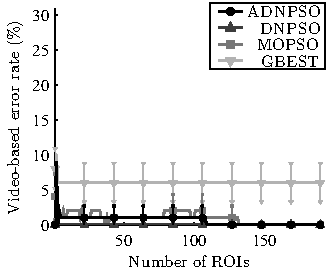
\includegraphics[width=0.31\linewidth]{c3_fig8a}  }
		\subfloat[$t=5$]{
		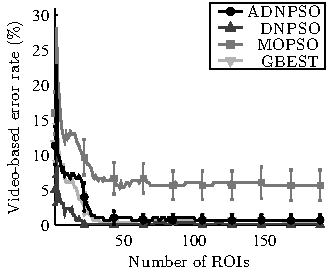
\includegraphics[width=0.31\linewidth]{c3_fig8b}  }
		\subfloat[$t=10$]{
		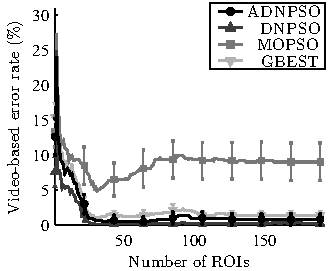
\includegraphics[width=0.31\linewidth]{c3_fig8c} } }
  	\caption{Evolution of the video-based error rate versus the number of ROIs used to identify individuals of the IIT-NRC data base during the \emph{enrollment} incremental learning scenario.
  Performance is shown at different points in time and error bars correspond to the 90\% confidence interval}
  \label{fig:c3_accAdd}
\end{figure*}
%--------------------- /Error rate - IIT-NRC, enrollment ----------------------%
%----------------------- Error rate - IIT-NRC, update -----------------------%
\begin{figure*}[t]
  \centering
  \fbox{
		\subfloat[$t=1$]{
		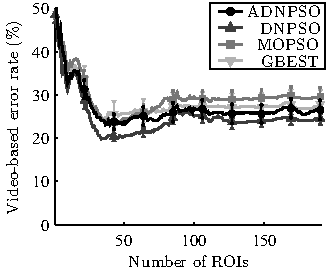
\includegraphics[width=0.31\linewidth]{c3_fig9a}  }
		\subfloat[$t=6$]{
		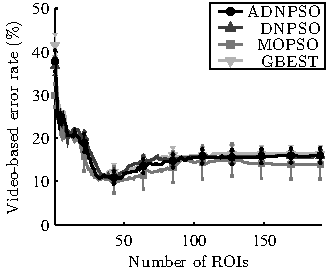
\includegraphics[width=0.31\linewidth]{c3_fig9b}  }
		\subfloat[$t=12$]{
		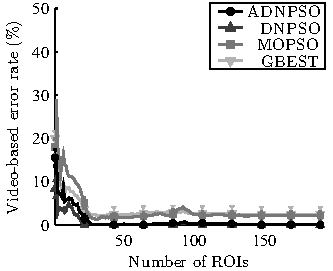
\includegraphics[width=0.31\linewidth]{c3_fig9c} } }
  	\caption{Evolution of the video-based error rate versus the number of ROIs used to identify individuals of the IIT-NRC data base during the \emph{update} incremental learning scenario.
  Performance is shown at different points in time and error bars correspond to the 90\% confidence interval}
  \label{fig:c3_accUpd}
\end{figure*}
%---------------------- /Error rate - IIT-NRC, update -----------------------%
%----------------------------- CMC - enrollment -------------------------------%
\begin{figure*}[t]
	\centering
  \fbox{
		\subfloat[$t=1$]{
		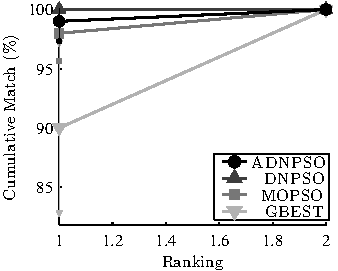
\includegraphics[width=0.31\linewidth]{c3_fig10a}  }
		\subfloat[$t=5$]{
		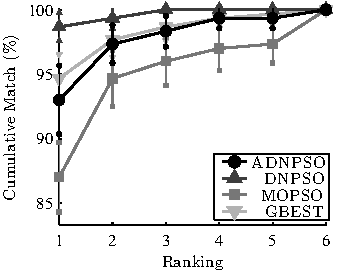
\includegraphics[width=0.31\linewidth]{c3_fig10b}  }
		\subfloat[$t=10$]{
		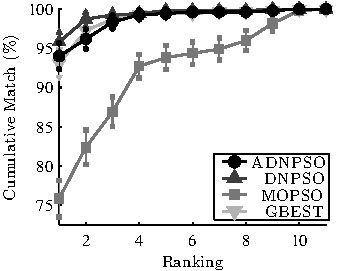
\includegraphics[width=0.31\linewidth]{c3_fig10c} } }
  	\caption{Cumulative match curves obtained during the \emph{enrollment} incremental learning scenario at different points in time when 15 ROIs are used to perform recognition.
  	Performance is shown at different points in time and error bars correspond to the 90\% confidence interval.
		During enrollment, the maximal rank increases with the number of classes present in the system}
  \label{fig:c3_cmcAdd}
\end{figure*}
%---------------------------- /CMC - enrollment -------------------------------%
%------------------------------- CMC - update ---------------------------------%
\begin{figure*}[t]
	\centering
  \fbox{
		\subfloat[$t=1$]{
		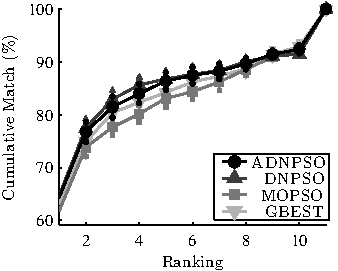
\includegraphics[width=0.31\linewidth]{c3_fig11a}  }
		\subfloat[$t=6$]{
		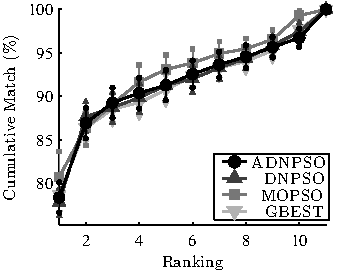
\includegraphics[width=0.31\linewidth]{c3_fig11b}  }
		\subfloat[$t=12$]{
		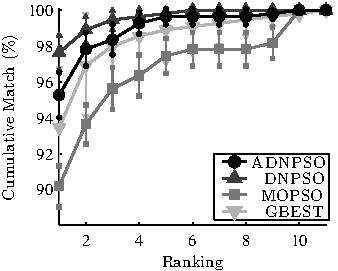
\includegraphics[width=0.31\linewidth]{c3_fig11c} } }
  	\caption{Cumulative match curves obtained during the \emph{update} incremental learning scenario at different points in time when 15 ROIs are used to perform recognition.
  	Performance is shown at different points in time and error bars correspond to the 90\% confidence interval.
		During enrollment, the maximal rank increases with the number of classes present in the system}
  \label{fig:c3_cmcUpd}
\end{figure*}
%------------------------------ /CMC - update ---------------------------------%

Figures \ref{fig:c3_accAdd} and \ref{fig:c3_accUpd} present the video-based generalization error rate according to the number of ROI used to perform recognition at different points in time for both incremental learning scenarios.
With each ROI, evidence in the form of FAM network outputs (binary codes) is accumulated and used to establish a ranking through majority voting.
When classes are enrolled incrementally, class decision boundaries become more complex in time.
Accuracy obtained with few ROIs then decreases, while the number of ROIs necessary to achieve a video-based error comparable to 0\% increases.
On the other hand, the video-based error rate obtained after updating classes through incremental learning decreases over time, as new blocks of data become available.
Moreover, when the AMCS has knowledge of the whole classification problem when adding new data, ensembles obtained are more robust as it can eventually achieve perfect accuracy.

When recognition is performed by accumulating responses of AMCSs over few ROI (15) during incremental learning, the cumulative match curves in Figures \ref{fig:c3_cmcAdd} and \ref{fig:c3_cmcUpd} are used to assess their ranking capabilities.
Ideally, with perfect accuracy, the correct class is always ranked first.
Ambiguity regarding predictions acts according to the error rate.
For the enrollment learning scenario, ranking capabilities diminishes in time when the classification environment becomes complex, and during update, it increases with the knowledge regarding individual class distributions.

However, when the number of ROIs used to perform recognition increases, the video-based error rate tends to increase at the end of each sequence.
When both learning and test sequences of the IIT-NRC data base were recorded, the individuals were all initially facing the camera, giving a full frontal image of their face.
As they start moving, changing his facial orientation and expression, different facial views, corresponding to data points in unexplored regions of the feature space, are presented to the system.
Recognizing an individual toward the end of a video sequence is thus more difficult.
Until all classes are updated, correct predictions for each ROI accumulated at the beginning of the test sequences are surpassed by the wrong predictions accumulated with the subsequent ROIs.

%------------ Number of ROIs necessary to achieve 100%, enrollment -----------%
\begin{table*}[t]
	\small
	\centering
		\caption{Minimal average error rate and number of ROIs necessary to achieve a generalization error rate \emph{comparable} to 0\% for video-based face recognition.
Results shown are obtained after learning the entire IIT-NRC and MoBo data bases through the both learning scenarios.
The mention ``never'' indicates that the method never achieves an error rate comparable to 0\%}
	\begin{tabular*}{\linewidth}{@{\extracolsep{\fill}}|l||rrrr||rr|}
		\hline
		Type of learning &\multicolumn{4}{c||}{Incremental} 
										 &\multicolumn{2}{c|}{Batch} \\
		Method	&ADNPSO &DNPSO &MOPSO &GBEST &PSO$_\text{B}$ &\textit{k}NN   \\\hline
		\multicolumn{7}{|l|}{\vspace{-5pt}}\\
		\multicolumn{7}{|l|}{\hspace{-5pt}\textbf{IIT-NRC data base}}	\\
		\multicolumn{7}{|l|}{\textit{Enrollment learning scenario}}		\\\hline
	  \hspace{15pt}Minimal av. error rate &$0.6\pm0.7$ &$0\pm0$ &$5\pm3$ 
																        &$2.1\pm1$ &$0\pm0$ &$0\pm0$ \\
	  \hspace{15pt}Nb. of ROIs to reach 0\% & 27    & 22 & never 
	  												  					  & never & 20 & 23    \\\hline

		\multicolumn{7}{|l|}{\textit{Update learning scenario}}\\\hline
	  \hspace{15pt}Minimal av. error rate &$0\pm0$ &$0\pm0$ &$1.2\pm0.6$ 
																    	  &$0.8\pm0.5$ &$0\pm0$ &$0\pm0$ \\
		\hspace{15pt}Nb. of ROIs to reach 0\% & 31     & 20 & never  
																				  & never  & 20 & 23    \\\hline

		\multicolumn{7}{|l|}{\vspace{-5pt}}\\
		\multicolumn{7}{|l|}{\hspace{-5pt}\textbf{MoBo data base}}	\\
		\multicolumn{7}{|l|}{\textit{Enrollment learning scenario}}		\\\hline
	  \hspace{15pt}Minimal av. error rate & $0\pm0$ & $0\pm0$ & $0.5\pm0.2$ 
																    	  & $1.2\pm1.4$ & $0\pm0$ & $0\pm0$ \\

		\hspace{15pt}Nb. of ROIs to reach 0\% & 30 & 28 & never & 25 & 30 & 16 \\\hline
		\multicolumn{7}{|l|}{\textit{Update learning scenario}}\\\hline

	  \hspace{15pt}Minimal av. error rate & $0\pm0$ & $0\pm0$ & $3\pm1$ 
															    	  & $0.3\pm0.3$ & $0\pm0$ & $0\pm0$ \\
		\hspace{15pt}Nb. of ROIs to reach 0\% & 27 & 24 & never & 25 & 30 & 16 
		\\\hline
	\end{tabular*}
	\label{tab:c3_accuracy}
\end{table*}
%----------- /Number of ROIs necessary to achieve 100%, enrollment -----------%

The accuracy of different methods are compared in Table \ref{tab:c3_accuracy} with the number ROIs needed to reach an error rate comparable to 0\% and the corresponding error rate.
The higher level of accuracy achieved by proposed AMCSs and a real time estimation on the speed a which this performance is attained.
An AMCS driven by ADNPSO can achieve a video-based error rate comparable to 0\% within a time frame similar to that obtained with mono-objective DNPSO incremental learning strategy and batch learning approaches.
In the worst case (the update scenario), the proposed method needs 10 additional ROIs than when mono-objective optimization is used with either incremental (DNPSO) or batch learning (PSO$_\text{B}$) to reach an error rate comparable to 0\%.
Assuming ideal tracking performances and a camera that acquires video sequences at a rate of 30 frames per second, this represents around a third of a second.
On the other hand, using MOO or the single global best solution during mono-objective optimization give less robust solutions and, in those cases, the AMCS's error rate is never comparable to 0\%.
Results are similar with the MoBo data base, except that AMCSs with the proposed DPSO-based strategy require fewer ROIs to achieve an error rate similar to 0\% and that a single FAM network can also achieve this level of accuracy.

%------------------ Comparison with others - MoBo and IIT-NRC -----------------%
\begin{table*}[t]
% 	\footnotesize
	\small
	\centering
	\caption{Comparison of the DPSO-based learning strategy with other authors on the IIT-NRC and MoBo data bases.
Classification rates were obtained for recognition on video sequences}
	\begin{tabular*}{\linewidth}{@{\extracolsep{\fill}}|l|lllll|}
		\hline
		\multicolumn{6}{|l|}{\vspace{-5pt}}\\
		\multicolumn{6}{|l|}{\textbf{IIT-NRC data base}}
		\\ \hline
		Proposed syst. & Arandjelovic et al. & Gorodnichy &
		Tangelder et al. & Wang et al. & \\
		& (2009) & (2005) & (2006) & (2009) & \\
		100\%  & 100\%  & $95\%$  & $95\%$  & $93\%$ & \\\hline
		
		\multicolumn{6}{|l|}{\vspace{-5pt}}\\
		\multicolumn{6}{|l|}{\hspace{-5pt}\textbf{MoBo data base}}				\\\hline
		Proposed syst. & Cevikalp et al. & Hadid et al. &  Liu et al. &
		Wang et al. & Zhou et al. \\
		& (2010) & (2004) & (2003) & (2008) & (2003) \\
		$100\%$  & $98\%$ & $94\%$  & $99\%$  & $94\%$  & $100\%$
		\\ \hline
	\end{tabular*}
	\label{tab:c3_vsOthers}
\end{table*}
%----------------- \Comparison with others - MoBo and IIT-NRC -----------------%


%------------------------------ Complexity - all ------------------------------%
\begin{table*}[t]
	\small
	\centering
	\caption{Structural complexity indicators of AMCSs that always give error rates comparable to 0\%.
Results are given after incremental learning of both data bases and learning scenarios.
Complexity is evaluated in terms of ensemble size, average network compression, and total compression of the entire ensemble.
The arrows serves as reminders that lower ensemble sizes and higher compressions indicate better results.
Each cell is presented with the 90\% confidence interval, and the best values are highlighted}
	\begin{tabular*}{\linewidth}{@{\extracolsep{\fill}}|l||rr||rr|}
		\hline
		Type of learning &\multicolumn{2}{c||}{Incremental} 
										 &\multicolumn{2}{c|}{Batch} \\ 
		Method	&\textbf{ADNPSO} &DNPSO &PSO$_\text{B}$ &\textit{k}NN   \\\hline
		
		\multicolumn{5}{|l|}{\vspace{-5pt}}\\
		\multicolumn{5}{|l|}{\hspace{-5pt}\textbf{IIT-NRC data base}}	\\
		\multicolumn{5}{|l|}{\textit{Enrollment learning scenario}}		\\\hline
		\hspace{15pt}
		Ensemble size ($\downarrow$)
			&$4.5\pm0.4$  &$19.4\pm0.7$   &$60\pm0$         &$\mathbf{1\pm0}$ \\
		\hspace{15pt}
		Average comp. ($\uparrow$)
      &$\mathbf{9.3\pm0.7}$  &$6.7\pm0.3$    &$2.2\pm0.2$      &$1\pm0$ \\
		\hspace{15pt}
		Total comp. ($\uparrow$)
			&$\mathbf{2.1\pm0.2}$  &$0.34\pm0.02$  &$0.037\pm0.003$  &$1\pm0$ \\\hline
																 
		\multicolumn{5}{|l|}{\vspace{-5pt}}\\
		\multicolumn{5}{|l|}{\textit{Update learning scenario}}
		\\ \hline
		\hspace{15pt}
 		Ensemble size ($\downarrow$)
			&$5.5\pm0.4$  &$19.5\pm0.7$   &$60\pm0$         &$\mathbf{1\pm0}$ \\
		\hspace{15pt}
 		Average comp. ($\uparrow$)
			&$\mathbf{7.4\pm0.4}$  &$5.8\pm0.2$    &$2.2\pm0.2$      &$1\pm0$ \\
		\hspace{15pt}
 		Total comp.   ($\uparrow$)
			&$\mathbf{1.4\pm0.2}$  &$0.30\pm0.03$  &$0.037\pm0.003$  &$1\pm0$ \\\hline

		\multicolumn{5}{|l|}{\vspace{-5pt}}\\
		\multicolumn{5}{|l|}{\hspace{-5pt}\textbf{MoBo data base}}	\\
		\multicolumn{5}{|l|}{\textit{Enrollment learning scenario}}	\\\hline
		\hspace{15pt}
		Ensemble size ($\downarrow$)
			&$7.5\pm0.5$  &$23.3\pm0.7$  &$60\pm0$         &$\mathbf{1\pm0}$ \\
		\hspace{15pt}
		Average comp. ($\uparrow$)
		&$\mathbf{50\pm6}$       &$23\pm2$	    &$3.6\pm0.1$      &$1\pm0$ \\
		\hspace{15pt}
		Total comp. ($\uparrow$)
			&$\mathbf{6.7\pm0.7}$  &$1.0\pm0.1$   &$0.060\pm0.004$  &$1\pm0$ \\\hline

		\multicolumn{5}{|l|}{\vspace{-5pt}}\\
		\multicolumn{5}{|l|}{\textit{Update learning scenario}}
		\\\hline
		\hspace{15pt}
		Ensemble size ($\downarrow$)
			&$5.5\pm0.8$           &$19.4\pm0.8$  &$60\pm0$       &$\mathbf{1\pm0}$ \\
		\hspace{15pt}
		Average comp. ($\uparrow$)
			&$\mathbf{28\pm1}$     &$18.6\pm0.8$  &$3.6\pm0.1$      &$1\pm0$ \\
		\hspace{15pt}
		Total comp. ($\uparrow$)
			&$\mathbf{5.1\pm0.5}$  &$0.9\pm0.1$   &$0.060\pm0.004$  &$1\pm0$ \\\hline
	\end{tabular*}
	\label{tab:c3_cpt}
\end{table*}
%----------------------------- /Complexity - all ------------------------------%

Table \ref{tab:c3_vsOthers} presents a comparison of accuracy obtained with other video-based face recognition systems in literature that perform \emph{batch learning} on both IIT-NRC and MoBo data bases.
With the exception of \cite{arandjelovic09} with the IIT-NRC data base and \cite{zhou03} with the MoBo data base, the AMCS with the proposed ADNPSO learning strategy outperforms all other systems. 
Regardless of the scenario, the AMCS with ADNPSO must accumulate about 1 second of video stream to achieve an error rate of 0\% after incremental learning of the entire MoBo data base.
In comparison, after performing \emph{batch learning} of the MoBo data base,
\cite{zhou03} achieved the same result by accumulating classifier responses for 0.5 second.
While \cite{arandjelovic09} also obtained a 0\% video-based error rate, the number of accumulated response, to achieve this is not available. 

Previous result showed that an AMCS driven by ADNPSO can achieve generalization capabilities comparable to 100\% with few ROIs.
Table \ref{tab:c3_cpt} depicts the structural complexity indicators only for ensembles that yielded error rates comparable to 0\%.
On this aspect, ADNPSO resulted in ensembles with less base classifiers, where the average structural complexity (compression) of each member is lower (higher), and thus less overall ensemble complexity.
Not only are ensembles smaller, but the average ensemble member obtained with ADNPSO uses only a fraction of the classifiers present in the archive.
Given the limited number of training samples available in the worst case (the update scenario), designing ensembles with all reference samples in the IIT-NRC and MoBo data bases yield ensembles composed of an average of $J=870$ and $J=5700$ $F_2$ layer nodes, respectively.
Each time a query sample is presented to the face recognition system, the FAM choice function (Equation \ref{eq:c3_choice}) is evaluated for each $F_2$ layer node.
For each query sample, FAM predictions have a time complexity of $O(IJ)$, where the number of input features has been fixed here to $I=64$.
For each camera with a frame rate of 30 frames per second in a moderately cluttered scene (ten people maximum), the system will process a worst case of 300 ROIs per second.
By today's standard this can be easily accomplished in 1/300 second on a standard desktop computer.%
\footnote{This statement is valid assuming a moderate number of individuals populating a scene and cameras feeding the face recognition system.}
 
Compared to the batch method learning methods, Table \ref{tab:c3_cpt} shows that incremental learning performed with PSO-based learning strategies provides simpler models that batch learning.
However, only the proposed ADNPSO gives comparable accuracy \emph{and} higher compression than \textit{k}NN after performing incremental learning on both data bases and during both scenarios.
Although ADNPSO and \textit{k}NN compressions are on the same scale, it should be noted that using the latter with $J$ recognition category (\emph{i.e.}, training samples) implies computing the Euclidean distance for each $J$ category and ranks the solutions to find the best $k$, a time complexity of $O(kI J\text{log}(J))$.


%------------------------------------------------------------------------------%
%--------------------------- Subsection - complexity --------------------------%
\subsection{Swarm and archive evolution during optimization}
\label{sec:c3_obj_space}

To give an example on how pools of classifier are generated and ensembles are selected, Figure \ref{fig:c3_updArc} gives an example of the swarm's evolution in the objective space during the update incremental learning scenario.
It compares mono-objective optimization (DNPSO), formal MOO (MOPSO), and the proposed ADNPSO scheme for the replication that yielded error rate for single ROIs closest to the average.

%-------------------------- Swarm & archive - update --------------------------%
\begin{figure*}[!t]
  \centering
  \fbox{\begin{minipage}{0.98\linewidth}
  \centering
\textbf{Mono-objective optimization with DNPSO and hypothetical classic archive}\\
\vspace{5pt}
		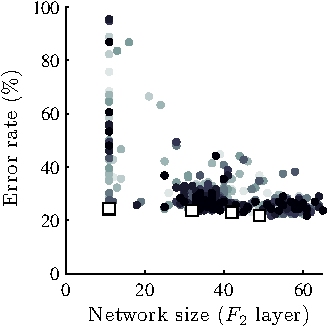
\includegraphics[width=0.31\linewidth]{c3_fig12a}\ \ 
		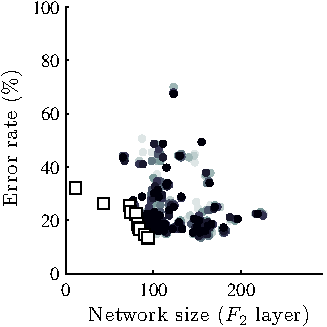
\includegraphics[width=0.31\linewidth]{c3_fig12b}\ \ 
		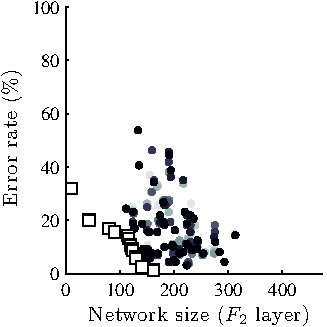
\includegraphics[width=0.31\linewidth]{c3_fig12c}\\
\vspace{5pt}
\textbf{MOO with MOPSO and classic archive}\\
		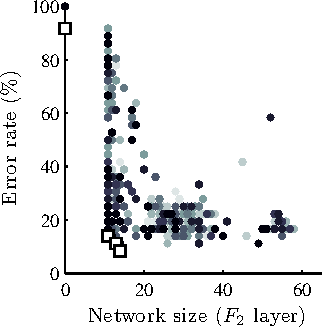
\includegraphics[width=0.31\linewidth]{c3_fig12d}\ \ 
		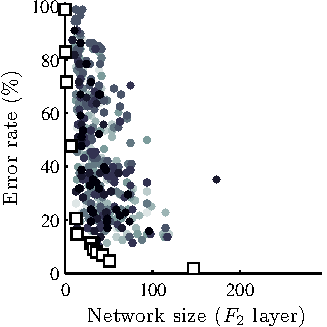
\includegraphics[width=0.31\linewidth]{c3_fig12e}\ \ 
		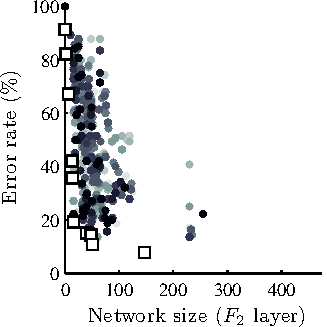
\includegraphics[width=0.31\linewidth]{c3_fig12f}\\
\vspace{5pt}
\textbf{ADNPSO with specialized archive}\\
		\subfloat[$t=1$]{  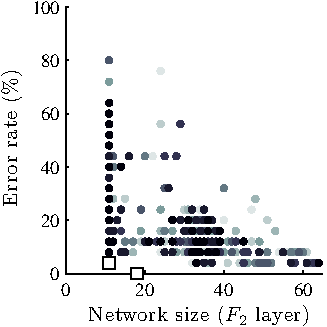
\includegraphics[width=0.31\linewidth]{c3_fig12g} }\ \ 
		\subfloat[$t=6$]{  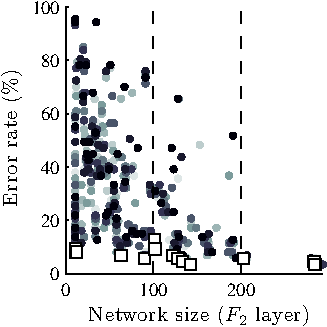
\includegraphics[width=0.31\linewidth]{c3_fig12h} }\ \ 
		\subfloat[$t=12$]{ 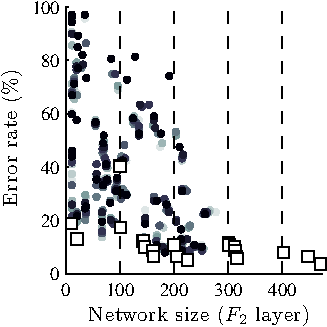
\includegraphics[width=0.31\linewidth]{c3_fig12i} }
  \end{minipage} }
  	\caption{Objective space during the update incremental learning scenario.
Circles show evolution of the swarm during its evolution at a time $t$, and squares illustrate solutions stored (or would be stored for mono-objective optimization) in the archive.
Light and dark circles respectively indicate the position of each particle at the start and end of the optimization process}
	\label{fig:c3_updArc}
\end{figure*}
%------------------------- /Swarm & archive - update --------------------------%

During mono-objective optimization with the DNPSO algorithm, networks in the swarm evolve according only to accuracy.
When learning data from complex classification environments, FAM networks then tend to continuously grow its $F_2$ layer to maintain or increase its accuracy.
The swarm then tends to move downward in the objective space, while neglecting the search for potential lighter solutions that could also provide networks accurate enough to be included in an ensemble.

If influences are define in the objective space with the MOSPO algorithm, Figure \ref{fig:c3_updArc} shows that using classifiers such as FAM introduces a bias in the swarm's movements toward structural complexity.
While the MOPSO algorithm theoretically considers both objectives equally, when used to evolve FAM networks, Figure \ref{fig:c3_updArc} shows that it is easier to find non-dominated solutions with smaller $F_2$ layer sizes than with lower error rate.
In time, the MOPSO algorithm directs most particles in the different search spaces such as mostly minimizing FAM $F_2$ layer size, thus limiting the search capabilities for accurate solutions.

On the other hand, the proposed ADNPSO directs subswarms of particles according to either accuracy, network size, or both at the same time (see Figure \ref{fig:c3_influences}).
Although this creates a swarm of particles that could successfully fill a classical archive, the specialized archive insures that the most accurate solutions of different network sizes are stored.
As results presented earlier showed, this creates suitable pools and ensembles of FAM neural networks.
Still, if several classes are added in time and the classification environment becomes more complex, it could become necessary to redefine the specialized archive's boundaries to accommodate such changes.

%------------------------------------------------------------------------------%
%------------------------------------------------------------------------------%
%------------------------------------------------------------------------------%
\section{Conclusion}
\label{sec:c3_conclusion}

In this chapter, an ADNPSO incremental learning strategy is proposed to evolve heterogeneous ensembles of classifiers in response to new reference data during video face recognition.
This strategy is applied to an AMCS where all parameters of a swarm of FAM neural network classifiers  (\emph{i.e.}, a swarm of classifiers), each one corresponding to a particle, are co-optimized such that both error rate and network size are minimized.
To provide a high level of accuracy over time while minimizing the computational complexity, the AMCS integrates information from multiple diverse classifiers, where learning is guided by an aggregated dynamical niching PSO (ADNPSO) algorithm that optimizes networks according both these objectives.
By using the specialized archive, local Pareto-optimal solutions detected by the ADNPSO algorithm can also be stored and combined with a greedy search algorithm to create ensembles based on accuracy, phenotype and genotype diversity.

Overall results indicates that using information in the search space of each objective (local optima positions and values), rather than in the objective space, permits creating pools of classifiers that are more accurate and with lower computational cost.
This results in ensembles that give an accuracy comparable to that obtained with mono-objective optimization and batch learning methods.
However, this is achieved with only a fraction of the computational cost (between 16\% and 20\% depending on the data base and learning scenario used).

However, the proposed AMCS is designed to observe small amounts of learning data under several perspectives with a swarm of classifiers, so that it can perform in the context of a real video-based face recognition application.
Although it can be performed off-line, while predictions can afterward be performed on-line, the learning process can become long when applied if data acquisition conditions are more constrained and data is available in large amounts (such as with the MoBo data base).
To circumvent this problem, future work should then consider focusing on 
characterizing reference learning samples with different quality measures.
To disambiguate concepts and further reduce FAM network structural complexity, available data could then be filtered according their level of quality so that learning is performed only with suitable samples.
In this context, the utility of the LTM used in the AMCS could also be redefined.
Rather than using the LTM only for validation purposes, it could also use these 
quality measures to select reference samples and keep a representative snapshot of the data distributions at a time $t$.
This way networks in the swarm could be reinitialized if they bring no new knowledge during the learning process.